% Aquest script fa el mateix que la versio anterior però he canviat 
% les dades de TCGA que em va donar el Diego per les descarregades de cBioportal 
% i les dades "TRUE" i "FALSE" de DA per les que he extret mostrejant

% Un canvi de darrera hora ha estat que, enlloc de fer servir les dades ajustades a tres bandes ("3-way"), hem conclos que no ens acabem de refiar de les dades d'RNAseq. Això vol dir que no ens cal treballar amb les dades 3-way sino que n'hi ha prou amb les 2-way que en el cas de microarrays i RNA-seq coincideixen en 30 mostres, enlloc de'n 25.

%També hem detectat un problema estrany consistent en que, en les dades de metilació que empravem, el gen que interessa al DIego, el ZBTB18, tenia els valors canviats, per la qual cosa hem pres dues decisions
% - Fer un pas enrrere i basar-nos en les dades gravades en binari
% - DEixar de fer servir les dadades de RNAseq (ja no ho feia) i basar l'anàlisi en les 30 linies celulars comunes entre Metilacio i Expressio enlloc de les 25 comunes entre els tres tipus de dades.

\documentclass[a4paper,10pt]{article}\usepackage[]{graphicx}\usepackage[]{color}
%% maxwidth is the original width if it is less than linewidth
%% otherwise use linewidth (to make sure the graphics do not exceed the margin)
\makeatletter
\def\maxwidth{ %
  \ifdim\Gin@nat@width>\linewidth
    \linewidth
  \else
    \Gin@nat@width
  \fi
}
\makeatother

\definecolor{fgcolor}{rgb}{0.345, 0.345, 0.345}
\newcommand{\hlnum}[1]{\textcolor[rgb]{0.686,0.059,0.569}{#1}}%
\newcommand{\hlstr}[1]{\textcolor[rgb]{0.192,0.494,0.8}{#1}}%
\newcommand{\hlcom}[1]{\textcolor[rgb]{0.678,0.584,0.686}{\textit{#1}}}%
\newcommand{\hlopt}[1]{\textcolor[rgb]{0,0,0}{#1}}%
\newcommand{\hlstd}[1]{\textcolor[rgb]{0.345,0.345,0.345}{#1}}%
\newcommand{\hlkwa}[1]{\textcolor[rgb]{0.161,0.373,0.58}{\textbf{#1}}}%
\newcommand{\hlkwb}[1]{\textcolor[rgb]{0.69,0.353,0.396}{#1}}%
\newcommand{\hlkwc}[1]{\textcolor[rgb]{0.333,0.667,0.333}{#1}}%
\newcommand{\hlkwd}[1]{\textcolor[rgb]{0.737,0.353,0.396}{\textbf{#1}}}%
\let\hlipl\hlkwb

\usepackage{framed}
\makeatletter
\newenvironment{kframe}{%
 \def\at@end@of@kframe{}%
 \ifinner\ifhmode%
  \def\at@end@of@kframe{\end{minipage}}%
  \begin{minipage}{\columnwidth}%
 \fi\fi%
 \def\FrameCommand##1{\hskip\@totalleftmargin \hskip-\fboxsep
 \colorbox{shadecolor}{##1}\hskip-\fboxsep
     % There is no \\@totalrightmargin, so:
     \hskip-\linewidth \hskip-\@totalleftmargin \hskip\columnwidth}%
 \MakeFramed {\advance\hsize-\width
   \@totalleftmargin\z@ \linewidth\hsize
   \@setminipage}}%
 {\par\unskip\endMakeFramed%
 \at@end@of@kframe}
\makeatother

\definecolor{shadecolor}{rgb}{.97, .97, .97}
\definecolor{messagecolor}{rgb}{0, 0, 0}
\definecolor{warningcolor}{rgb}{1, 0, 1}
\definecolor{errorcolor}{rgb}{1, 0, 0}
\newenvironment{knitrout}{}{} % an empty environment to be redefined in TeX

\usepackage{alltt}
\usepackage[T1]{fontenc}
%\usepackage[utf8]{inputenc}
%\usepackage[spanish]{babel}
\usepackage{url}
\usepackage{amsmath}
\usepackage{amssymb}
\usepackage{amsfonts}
\usepackage{underscore}
%\usepackage{graphicx}
%\usepackage{pstricks}

\setlength{\oddsidemargin}{0pt} \setlength{\evensidemargin}{0pt}
\setlength{\marginparwidth}{1in} \setlength{\marginparsep}{0pt}

\setlength{\topmargin}{0pt} \setlength{\headheight}{0pt}
\setlength{\headsep}{0pt} \setlength{\topskip}{0pt}

% \footheight 0pt
% \footskip 0pt
% A4 is 29,7301778cm x 21,0224103cm
%     =  9,7047944in x 6,2765395in
\setlength{\textheight}{24,6501778cm}
\setlength{\textwidth}{15,9424103cm}

\setlength{\parindent}{0pt}

\pagestyle{plain}

\title{Scatterplot analysis for the integrative analysis of expression and methylation data}
\author{S\'anchez-Pla, Alex$^{1,3}$, Mir\'o, Berta$^3$, Carmona, Francesc$^1$, \\ Bazzoco, Sara$^2$, Arango, Diego$^2$\\
  $^1$ Departament of Genetics Microbiology and Statistics, Universitat de Barcelona\\
  $^2$ CIBBIM-Nanomedicine. Biomedical Research in Digestive Tumors, (VHIR), Barcelona\\
  $^3$ Statistic and Bioinformatics Unit. Vall d'Hebron Research Institute.  (VHIR). Barcelona}
\date{}
\IfFileExists{upquote.sty}{\usepackage{upquote}}{}
\begin{document}



\maketitle

\thispagestyle{empty}

\tableofcontents

\section{Introduction}

This document describes how to implement a pipeline for selecting L-shaped genes from two data matrices, an expression and a methylation matrix, matched by rows (genes) and columns(samples), using the algorithms implemented by the authors and described elsewhere.

The idea is to "keep-it-simple" so that it the process can be followed by a non-technical reader. 

The steps correpond roughly to what one user would do when exploring two expression-methylation datasets

\begin{enumerate}
  \item Data input: For each dataset
  \begin{enumerate} 
    \item Select (Load) expression values from a csv (or binary) file
    \item Select (Load) methylation values from a csv  (or binary) file
    \item Check that the data are well composed and matched
  \end{enumerate}
  \item For each selection method (Naïve, CMI, Heuristic)
  \begin{enumerate}
   \item Set parameters if needed)
    \item Compute binary and numeric scores to for each gene
    \item Output result in tab format: geneId, NumScore, binScore
  \end{enumerate}
  This will yield a results table (a list) for each method.
  \item Define consensus list of l-shaped genes (e.g. by intersection or union or selection of output L-lists)
  \item Plot consensus lists scatterplots
  \item Compute genome positions of selected genes and
  \begin{enumerate}
  \item Plot genes in chromosome
  \item Add gene positions to results table
  \end{enumerate}
  \item Do enrichment analysis of the selecte gene list
\end{enumerate}








\begin{knitrout}
\definecolor{shadecolor}{rgb}{0.969, 0.969, 0.969}\color{fgcolor}\begin{kframe}
\begin{verbatim}
## NULL
\end{verbatim}
\end{kframe}
\end{knitrout}



\begin{knitrout}
\definecolor{shadecolor}{rgb}{0.969, 0.969, 0.969}\color{fgcolor}\begin{kframe}
\begin{alltt}
\hlkwd{addToLinksFile}\hlstd{(}\hlstr{"GRMSelectionPipeline.csv"}\hlstd{,} \hlstr{"Informe"}\hlstd{)}
\end{alltt}
\end{kframe}
\end{knitrout}

\section{Datasets used for the study}

\subsection{On the preprocessing and selection of the researcher's data}

In a first version of this analysis the data for microarrays, RNAseq and methylation were used. 

In further analyses we have concluded that RNAseq data were less reliable than microarray data so that we decided to omit RNAseq data from then on. 

As a consequence we can use what we called "2 way data" that is, data that have been matched by pairs which have 30 instead of 25 samples.

The preprocessing of the data of microarrays and methylation was done in 3 processes:
\begin{enumerate}
\item \texttt{CorrelationAnalysis0New-ReadAndPreprocessDataV2}
\item  \texttt{CorrelationAnalysis1NEW-MatchData}
\item \texttt{CorrelationAnalysis2NEW-ComputeCorrs}
\end{enumerate}

The analysis performed in \texttt{CorrelationAnalysis0New-ReadAndPreprocessDataV2} has produced two methylation datasets. One where cpgs have been unitized to genes by averaging their values and another where this has been done by taking the probe with highest variance.

The analysis performed in \texttt{CorrelationAnalysis1NEW-MatchData}
has selected common genes and common samples between methylation and microarray data. Datasets \texttt{dataMarrCR2}, \texttt{dataMethCR2} and \texttt{dataMethVarCR2} contain microarray expression and methylation (unitized by mean and by variance) data matched by gene and samples. These datasets have been saved into a binary file: \texttt{matchedMarrRNAseqMethDataByPAIRS.Rda} and written separately to files \texttt{matched2MicroarrayData.csv}, \texttt{matched2MethylationData.csv} and \texttt{matched2MethVar.csv}.

\textbf{These will be the datasets used as "researcher's data in the analyses}

\subsection{Colon Cancer datasets}

There are three\footnote{An RNAseq dataset was also available but we decided not to use it because we were unsure of how reliable the values were} datasets available for analysis obtained from three sources. The first dataset has been obtained by the researcher, (Diego Arango) and will be named as \texttt{DA}. A second one, which we name as \texttt{GEO}, has been extracted from the Gene Expression Omnibus and the third dataset is the Colon Cancer dataset from The Cancer Genome Atlas project and will be designated as \texttt{TCGA}.

\begin{enumerate}
  \item \texttt{DA}: Expression microarrays (\texttt{matched2MicroarrayData.csv}) and Illumina 25k methylation arrays (\texttt{matched2MicroarrayData.csv}) on 30 cell llines.
  \item \texttt{GEO}: Expression microarrays (\texttt{geoMicroarrays.csv}) and Illumina 25k methylation arrays (\texttt{geoMetilacion.csv}) on 25 CRC samples.
\item  TCGA. Expression microarrays (\texttt{TCGAExprData.csv}) and Illumina 25k methylation arrays (\texttt{TCGAMetilData.csv}) on 426 Colon Adenocarcinoma (\texttt{COAD} dataset) samples from TCGA.
\end{enumerate}

A summary of each datasets follows below:
\begin{itemize}
\item \texttt{DA} dataset has been provided by the researcher (DA=``Diego Arango'') and is the original dataset on which it was intended to select L-shaped  genes.

\begin{knitrout}
\definecolor{shadecolor}{rgb}{0.969, 0.969, 0.969}\color{fgcolor}\begin{kframe}
\begin{alltt}
\hlkwd{require}\hlstd{(printr)}
\hlkwd{load}\hlstd{(}\hlkwd{file.path}\hlstd{(dadesDir,}\hlstr{"matchedMarrRNAseqMethDataByPAIRS.Rda"}\hlstd{))}
\hlstd{DAExprData} \hlkwb{<-} \hlkwd{as.matrix}\hlstd{(dataMarrCR2)}
\hlstd{DAMetilData} \hlkwb{<-} \hlkwd{as.matrix}\hlstd{(dataMethCR2)}
\hlkwd{rm}\hlstd{(dataMarrCR0,dataMarrCR2, dataMethCR1, dataMethCR2, dataMethVarCR1, dataMethVarCR2, dataRNAseqCR0, dataRNAseqCR0CS, dataRNAseqCR1, dataRNAseqCR1CS)} \hlcom{# clean files loaded with the desired files}
\hlcom{#write.csv2(DAExprData, file=file.path(dadesDir,"DatosMicroarrays.csv"),row.names = TRUE)}
\hlcom{# write.csv2(DAMetilData, file=file.path(dadesDir,"DatosMetilacion.csv"),row.names = TRUE)}
\hlcom{# DAExprData <- as.matrix(read.table(file=file.path(dadesDir,"DatosMicroarrays.csv"), header=TRUE, sep=";", dec=",", row.names = 1))}
\hlcom{# DAMetilData <- as.matrix(read.table(file=file.path(dadesDir,"DatosMetilacion.csv"), header=TRUE, sep=";",dec=",", row.names = 1))}
\hlcom{# DARNAseqData <- as.matrix(read.table(file=file.path(dadesDir,"DatosRNAseq.csv"), header=TRUE, sep=";",dec=",", row.names = 1))}
\hlkwd{cat}\hlstd{(}\hlstr{"DA Microarray data : "}\hlstd{,} \hlkwd{dim}\hlstd{(DAExprData),} \hlstr{"\textbackslash{}n"}\hlstd{)}
\end{alltt}
\begin{verbatim}
## DA Microarray data :  11359 30
\end{verbatim}
\begin{alltt}
\hlkwd{cat}\hlstd{(}\hlstr{"DA Methylation data: "}\hlstd{,} \hlkwd{dim}\hlstd{(DAMetilData),} \hlstr{"\textbackslash{}n"}\hlstd{)}
\end{alltt}
\begin{verbatim}
## DA Methylation data:  11359 30
\end{verbatim}
\begin{alltt}
\hlcom{# cat("DA RNASeq data     : ", dim(DARNAseqData), "\textbackslash{}n")}
\end{alltt}
\end{kframe}
\end{knitrout}

\item \texttt{geo} dataset is formed by data from expression microarrays (Illumina beadchips, \texttt{geoMicroarrays.csv}) and methylation array (Illumina 25kMethArray, \texttt{geoMetilacion.csv}) on 25 CRC samples. The data have been collected from the GEO database records: GSE25062 for the methylation data and GSE25070 for the expression data. The dataset has been created by taking the expression values available for 26 CRC tumors and matching with their corresponding methylation values.

\begin{knitrout}
\definecolor{shadecolor}{rgb}{0.969, 0.969, 0.969}\color{fgcolor}\begin{kframe}
\begin{alltt}
\hlstd{geoExprData} \hlkwb{<-}  \hlkwd{as.matrix}\hlstd{(}\hlkwd{read.table}\hlstd{(}\hlkwc{file}\hlstd{=}\hlkwd{file.path}\hlstd{(dadesDir,}\hlstr{"GEOExpData.csv"}\hlstd{),} \hlkwc{header}\hlstd{=}\hlnum{TRUE}\hlstd{,} \hlkwc{sep}\hlstd{=}\hlstr{";"}\hlstd{,} \hlkwc{dec}\hlstd{=}\hlstr{"."}\hlstd{))}
\hlstd{geoMetilData} \hlkwb{<-}  \hlkwd{as.matrix}\hlstd{(}\hlkwd{read.table}\hlstd{(}\hlkwc{file}\hlstd{=}\hlkwd{file.path}\hlstd{(dadesDir,}\hlstr{"GEOMethData.csv"}\hlstd{),} \hlkwc{header}\hlstd{=}\hlnum{TRUE}\hlstd{,} \hlkwc{sep}\hlstd{=}\hlstr{";"}\hlstd{,} \hlkwc{dec}\hlstd{=}\hlstr{"."}\hlstd{))}
\hlkwd{cat}\hlstd{(}\hlstr{"GEO Microarray data : "}\hlstd{,} \hlkwd{dim}\hlstd{(geoExprData),} \hlstr{"\textbackslash{}n"}\hlstd{)}
\end{alltt}
\begin{verbatim}
## GEO Microarray data :  11191 25
\end{verbatim}
\begin{alltt}
\hlkwd{cat}\hlstd{(}\hlstr{"GEO Methylation data: "}\hlstd{,} \hlkwd{dim}\hlstd{(geoMetilData),} \hlstr{"\textbackslash{}n"}\hlstd{)}
\end{alltt}
\begin{verbatim}
## GEO Methylation data:  11191 25
\end{verbatim}
\end{kframe}
\end{knitrout}

\item \texttt{TCGA} dataset has been obtained from The Cancer Genome Atlas Database (TCGA) (Colon Adenocarcinoma (\texttt{COAD}) Nature 2012 dataset) and downloaded through the cBioportal website.

\begin{knitrout}
\definecolor{shadecolor}{rgb}{0.969, 0.969, 0.969}\color{fgcolor}\begin{kframe}
\begin{alltt}
\hlstd{TCGAExprData} \hlkwb{<-}  \hlkwd{as.matrix}\hlstd{(}\hlkwd{read.table}\hlstd{(}\hlkwc{file}\hlstd{=}\hlstr{"dades/TCGA-cBioPortal-Expressions.csv"}\hlstd{,} \hlkwc{header}\hlstd{=}\hlnum{TRUE}\hlstd{,} \hlkwc{sep}\hlstd{=}\hlstr{","}\hlstd{,} \hlkwc{dec}\hlstd{=}\hlstr{"."}\hlstd{,} \hlkwc{row.names}\hlstd{=}\hlnum{1}\hlstd{))}
\hlstd{TCGAMetilData} \hlkwb{<-}  \hlkwd{as.matrix}\hlstd{(}\hlkwd{read.csv}\hlstd{(}\hlkwc{file}\hlstd{=}\hlstr{"dades/TCGA-cBioPortal-Methylations.csv"}\hlstd{,} \hlkwc{header}\hlstd{=}\hlnum{TRUE}\hlstd{,} \hlkwc{sep}\hlstd{=}\hlstr{","}\hlstd{,} \hlkwc{dec}\hlstd{=}\hlstr{"."}\hlstd{,} \hlkwc{row.names}\hlstd{=}\hlnum{1}\hlstd{))}
\hlkwd{cat}\hlstd{(}\hlstr{"TCGA Microarray data : "}\hlstd{,} \hlkwd{dim}\hlstd{(TCGAExprData),} \hlstr{"\textbackslash{}n"}\hlstd{)}
\end{alltt}
\begin{verbatim}
## TCGA Microarray data :  11788 223
\end{verbatim}
\begin{alltt}
\hlkwd{cat}\hlstd{(}\hlstr{"TCGA Methylation data: "}\hlstd{,} \hlkwd{dim}\hlstd{(TCGAMetilData),} \hlstr{"\textbackslash{}n"}\hlstd{)}
\end{alltt}
\begin{verbatim}
## TCGA Methylation data:  11788 223
\end{verbatim}
\end{kframe}
\end{knitrout}
\end{itemize}

\begin{knitrout}
\definecolor{shadecolor}{rgb}{0.969, 0.969, 0.969}\color{fgcolor}\begin{kframe}
\begin{alltt}
\hlstd{inCommon}\hlkwb{<-} \hlkwd{length}\hlstd{(}\hlkwd{intersect}\hlstd{(}\hlkwd{rownames}\hlstd{(DAExprData),} \hlkwd{rownames}\hlstd{(geoExprData)))}
\hlstd{inCommon2} \hlkwb{<-} \hlkwd{length}\hlstd{(}\hlkwd{intersect}\hlstd{(}\hlkwd{rownames}\hlstd{(DAExprData),} \hlkwd{rownames}\hlstd{(TCGAExprData)))}
\hlstd{inCommon3} \hlkwb{<-} \hlkwd{length}\hlstd{(}\hlkwd{intersect}\hlstd{(}\hlkwd{rownames}\hlstd{(geoExprData),} \hlkwd{rownames}\hlstd{(TCGAExprData)))}
\end{alltt}
\end{kframe}
\end{knitrout}

There are 9070 genes in common between the DAX dataset and the GEO datasets. There are 9876 common genes between the DAX dataset and the TCGA dataset and 8546 common genes between the GEO dataset and the TCGA dataset.

This can be visualized using a Venn diagram
\begin{knitrout}
\definecolor{shadecolor}{rgb}{0.969, 0.969, 0.969}\color{fgcolor}\begin{kframe}
\begin{alltt}
\hlstd{myVenn4} \hlkwb{<-} \hlkwd{venn.diagram}\hlstd{(}\hlkwc{x}\hlstd{=}\hlkwd{list}\hlstd{(}\hlkwc{DA}\hlstd{=}\hlkwd{rownames}\hlstd{(DAExprData),}
                              \hlkwc{GEO}\hlstd{=}\hlkwd{rownames}\hlstd{(geoExprData),}
                              \hlkwc{TCGA}\hlstd{=}\hlkwd{rownames}\hlstd{(TCGAExprData)),}
                              \hlkwc{filename}\hlstd{=}\hlkwa{NULL}\hlstd{,} \hlkwc{lty} \hlstd{=} \hlstr{"blank"}\hlstd{,}
                              \hlkwc{fill}\hlstd{=}\hlkwd{c}\hlstd{(}\hlstr{"pink1"}\hlstd{,} \hlstr{"skyblue"}\hlstd{,} \hlstr{"mediumorchid"}\hlstd{),}
                       \hlkwc{main}\hlstd{=}\hlstr{"Genes in common between the three datasets"}\hlstd{)}
\hlkwd{grid.newpage}\hlstd{()}
\hlkwd{grid.draw}\hlstd{(myVenn4)}
\end{alltt}
\end{kframe}
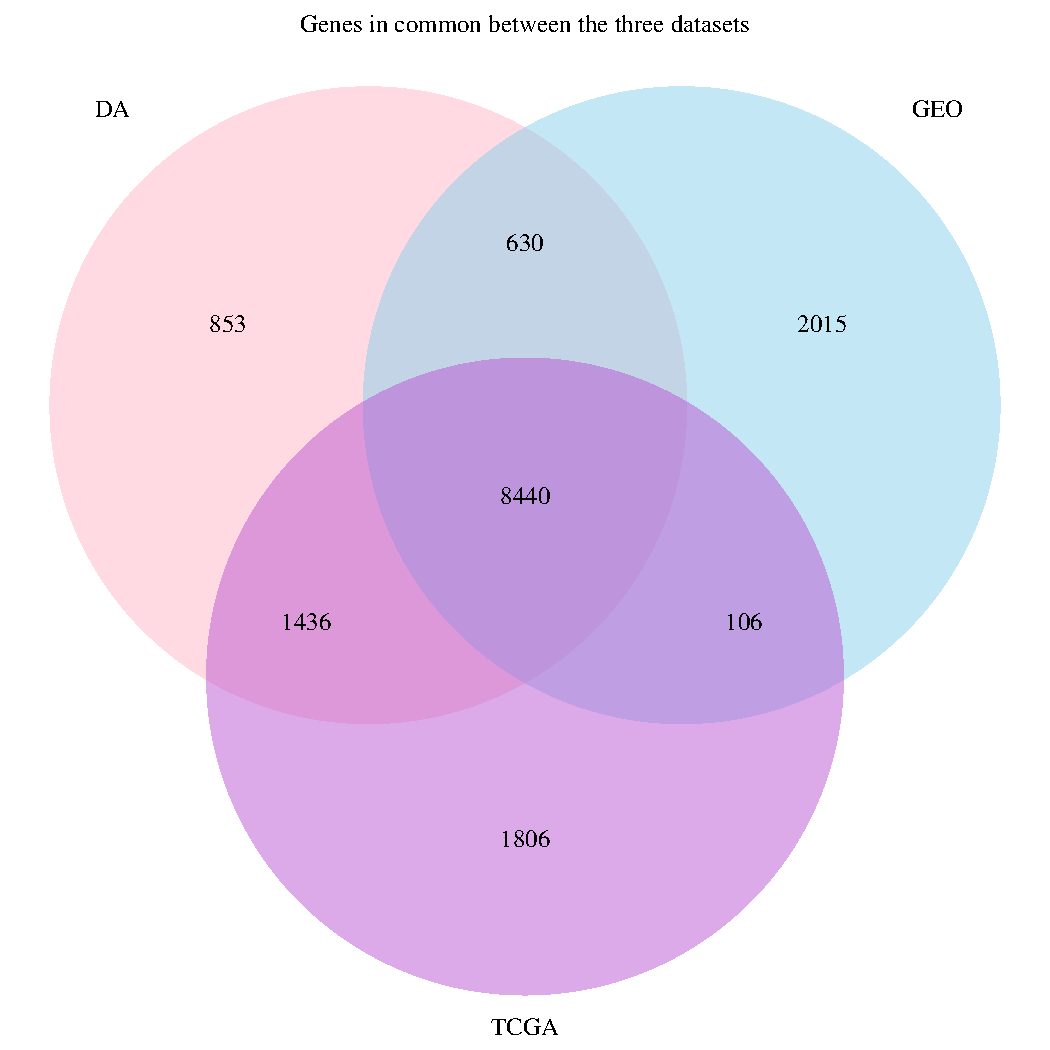
\includegraphics[width=\maxwidth]{figure/vennCommonGenesin3lists-1} 

\end{knitrout}

\subsection{TRUE and FALSE 'L-shaped' genes}

A problem with this study is that truly or falsely positive L-shaped genes are not known.

In the absence of this a list of \emph{apparently truly positive} and \emph{apparently truly negative} genes has been provided by the researcher.

\begin{knitrout}
\definecolor{shadecolor}{rgb}{0.969, 0.969, 0.969}\color{fgcolor}\begin{kframe}
\begin{alltt}
\hlcom{# Genes True i False}
\hlstd{trueLGeneDF} \hlkwb{<-}\hlkwd{read.table}\hlstd{(}\hlstr{"dades/genesTrueLNEW.txt"}\hlstd{)}
\hlstd{(trueLGeneNames} \hlkwb{<-} \hlkwd{as.character}\hlstd{(trueLGeneDF[,}\hlnum{1}\hlstd{]))}
\end{alltt}
\begin{verbatim}
##  [1] "ABCG2"      "ADH6"       "AKR1C4"     "BCL11B"     "CA9"       
##  [6] "CCR6"       "CST7"       "CX3CL1"     "DAPP1"      "CYP27A1"   
## [11] "ELAVL2"     "FAM84A"     "GREM1"      "HSD17B2"    "INHBB"     
## [16] "KCNV1"      "LHFP"       "MEP1A"      "LRP2"       "MAGEE1"    
## [21] "MEP1A"      "MYT1"       "NOX1"       "OAS2"       "PHYHIPL"   
## [26] "POF1B"      "POPDC3"     "PRDM16"     "PRDM5"      "QPCT"      
## [31] "RASGRF2"    "RAB6B"      "RASEF"      "RNF186"     "SOX2"      
## [36] "SOSTDC1"    "SPON1"      "ST6GALNAC1" "STEAP4"     "STK33"     
## [41] "TAPBPL"     "SYN2"       "THRB"       "TRAM1L1"    "WNK4"
\end{verbatim}
\begin{alltt}
\hlstd{falseLGeneDF} \hlkwb{<-} \hlkwd{read.table}\hlstd{(}\hlstr{"dades/genesFalseLNEW.txt"}\hlstd{)}
\hlstd{(falseLGeneNames} \hlkwb{<-} \hlkwd{as.character}\hlstd{(falseLGeneDF[,}\hlnum{1}\hlstd{]))}
\end{alltt}
\begin{verbatim}
##  [1] "ACOX2"     "ADA"       "AKR1B1"    "ALDH1A3"   "AMT"      
##  [6] "ANXA3"     "ARHGAP4"   "ARL14"     "ATP6AP2"   "AUTS2"    
## [11] "BHLHB9"    "BMP7"      "C19orf33"  "C1QTNF6"   "CAB39L"   
## [16] "CDH17"     "CDX1"      "CFTR"      "CIDEB"     "CMTM3"    
## [21] "DNAJA4"    "DUSP9"     "ELF3"      "ELMO3"     "FBP1"     
## [26] "FGD4"      "FKBP10"    "FOXC1"     "FUCA2"     "GNG4"     
## [31] "GPRC5A"    "GRAMD3"    "H1F0"      "HIST1H2BH" "HNMT"     
## [36] "HOOK1"     "HOOK3"     "HOXB3"     "HOXB2"     "HOXB5"    
## [41] "HS3ST1"    "LCMT2"     "LAMA3"     "LDHB"
\end{verbatim}
\begin{alltt}
\hlstd{trueLExpr} \hlkwb{<-} \hlstd{DAExprData[}\hlkwd{rownames}\hlstd{(DAExprData)} \hlopt \hlstd{trueLGeneNames ,]}
\hlstd{falseLExpr} \hlkwb{<-} \hlstd{DAExprData[}\hlkwd{rownames}\hlstd{(DAExprData)} \hlopt \hlstd{falseLGeneNames ,]}
\hlstd{trueLMet} \hlkwb{<-} \hlstd{DAMetilData[}\hlkwd{rownames}\hlstd{(DAMetilData)} \hlopt \hlstd{trueLGeneNames ,]}
\hlstd{falseLMet} \hlkwb{<-} \hlstd{DAMetilData[}\hlkwd{rownames}\hlstd{(DAMetilData)} \hlopt \hlstd{falseLGeneNames ,]}
\hlstd{DATrueFalseExpr} \hlkwb{<-} \hlkwd{as.matrix}\hlstd{(}\hlkwd{rbind}\hlstd{(trueLExpr, falseLExpr))}
\hlstd{DATrueFalseMet} \hlkwb{<-} \hlkwd{as.matrix}\hlstd{(}\hlkwd{rbind}\hlstd{(trueLMet, falseLMet))}
\end{alltt}
\end{kframe}
\end{knitrout}


\subsection{Additional data checks}

The data for these analyses must have a common structure: \textbf{Each pair of matrices (Expression-Methylation) must have the same rome and column names}, that is both datasets must contain information for the same genes and same samples at their corresponding positions.

This can be checked using a simple function such as \texttt{checkData} available in the package.
\begin{knitrout}
\definecolor{shadecolor}{rgb}{0.969, 0.969, 0.969}\color{fgcolor}\begin{kframe}
\begin{alltt}
\hlkwd{try}\hlstd{(}\hlkwa{if}\hlstd{(}\hlopt{!}\hlkwd{checkPairing}\hlstd{(DAExprData, DAMetilData))} \hlkwd{stop}\hlstd{(}\hlstr{"Row names and/or column names do not match"}\hlstd{))}
\hlkwd{try}\hlstd{(}\hlkwa{if}\hlstd{(}\hlopt{!}\hlkwd{checkPairing}\hlstd{(geoExprData, geoMetilData))} \hlkwd{stop}\hlstd{(}\hlstr{"Row names and/or column names do not match"}\hlstd{))}
\hlkwd{try}\hlstd{(}\hlkwa{if}\hlstd{(}\hlopt{!}\hlkwd{checkPairing}\hlstd{(TCGAExprData, TCGAMetilData))} \hlkwd{stop}\hlstd{(}\hlstr{"Row names and/or column names do not match"}\hlstd{))}
\hlkwd{try}\hlstd{(}\hlkwa{if}\hlstd{(}\hlopt{!}\hlkwd{checkPairing}\hlstd{(trueLExpr, trueLMet))} \hlkwd{stop}\hlstd{(}\hlstr{"Row names and/or column names do not match"}\hlstd{))}
\hlkwd{try}\hlstd{(}\hlkwa{if}\hlstd{(}\hlopt{!}\hlkwd{checkPairing}\hlstd{(falseLExpr, falseLMet))} \hlkwd{stop}\hlstd{(}\hlstr{"Row names and/or column names do not match"}\hlstd{))}
\hlkwd{try}\hlstd{(}\hlkwa{if}\hlstd{(}\hlopt{!}\hlkwd{checkPairing}\hlstd{(DATrueFalseExpr, DATrueFalseMet))} \hlkwd{stop}\hlstd{(}\hlstr{"Row names and/or column names do not match"}\hlstd{))}
\end{alltt}
\end{kframe}
\end{knitrout}

\section{Selection of L-shaped genes}
\subsection{Methods}
After a long process of trial and error we consider that there are three ``best'' approaches for selecting L-shaped genes. The methods are extensively described in another document so only a brief description is provided below:
\begin{enumerate}
  \item \textbf{Naive}: A gene is called L-shaped if Methylation and expression are significantly negatively correlated. 
  \item \textbf{CMI}: A gene is called L-Shaped if the \emph{Conditional Mutual Information} (CMI) of the expression and methylation values computed at different points between 0 and 1 reaches a minimum  which is small enough according predefined thresholds. This minimum can be considered to be the cutoff for methylation.
  \item \textbf{Heuristic}: A gene is called L-shaped if the majority of the points of the scatterplot stay on the left and lower cells of a $3\times3$ grid. How many values can deviate from this "majority" in each cell can be tuned by the user.
\end{enumerate}

\subsection{Selecting L-shaped genes with the Naive method}

A gene is called L-shaped if methylation and expression are significantly negatively correlated. If the number of samples is big, as in the TCGA dataset, many genes will be significantly correlated. In these cases it may be worth to set an additional threshold such as $r < -0.XXX$ where $-0.XXX$ is a threshold to be set by the user. A trial and error process suggests that a -0.5 cutoff may be appropriate

\begin{knitrout}
\definecolor{shadecolor}{rgb}{0.969, 0.969, 0.969}\color{fgcolor}\begin{kframe}
\begin{alltt}
\hlcom{#calcAgain <- TRUE}
\hlcom{#if (!file.exists("results/naiveSelections.Rda") || calcAgain)\{}
\hlstd{naiveDA} \hlkwb{<-} \hlkwd{naiveSelection} \hlstd{(DAExprData, DAMetilData,} \hlkwc{pValCutoff}\hlstd{=}\hlnum{0.25}\hlstd{,} \hlkwc{rCutoff}\hlstd{=}\hlopt{-}\hlnum{0.5}\hlstd{,} \hlkwc{type}\hlstd{=}\hlstr{"Spearman"}\hlstd{,}\hlkwc{adj}\hlstd{=}\hlnum{TRUE}\hlstd{)}
\hlstd{selectedNaiveDA} \hlkwb{<-}\hlstd{naiveDA[naiveDA}\hlopt{$}\hlstd{SigNegCorr,]}
\end{alltt}
\end{kframe}
\end{knitrout}

\begin{knitrout}
\definecolor{shadecolor}{rgb}{0.969, 0.969, 0.969}\color{fgcolor}\begin{kframe}
\begin{alltt}
    \hlstd{naiveGEO} \hlkwb{<-} \hlkwd{naiveSelection} \hlstd{(geoExprData, geoMetilData,} \hlkwc{pValCutoff}\hlstd{=}\hlnum{0.25}\hlstd{,}  \hlkwc{rCutoff}\hlstd{=}\hlopt{-}\hlnum{0.5}\hlstd{,} \hlkwc{type}\hlstd{=}\hlstr{"Spearman"}\hlstd{,} \hlkwc{adj}\hlstd{=}\hlnum{TRUE}\hlstd{)}
    \hlstd{selectedNaiveGEO} \hlkwb{<-}\hlstd{naiveGEO[naiveGEO}\hlopt{$}\hlstd{SigNegCorr,]}
\end{alltt}
\end{kframe}
\end{knitrout}
\begin{knitrout}
\definecolor{shadecolor}{rgb}{0.969, 0.969, 0.969}\color{fgcolor}\begin{kframe}
\begin{alltt}
\hlstd{naiveTCGA} \hlkwb{<-} \hlkwd{naiveSelection} \hlstd{(TCGAExprData, TCGAMetilData,} \hlkwc{pValCutoff}\hlstd{=}\hlnum{0.25}\hlstd{,}  \hlkwc{rCutoff}\hlstd{=}\hlopt{-}\hlnum{0.5}\hlstd{,} \hlkwc{type}\hlstd{=}\hlstr{"Spearman"}\hlstd{,} \hlkwc{adj}\hlstd{=}\hlnum{TRUE}\hlstd{)}
\hlstd{selectedNaiveTCGA} \hlkwb{<-}\hlstd{naiveTCGA[naiveTCGA}\hlopt{$}\hlstd{SigNegCorr,]}
\end{alltt}
\end{kframe}
\end{knitrout}

\begin{knitrout}
\definecolor{shadecolor}{rgb}{0.969, 0.969, 0.969}\color{fgcolor}\begin{kframe}
\begin{alltt}
\hlkwd{save}\hlstd{(naiveDA, naiveGEO, naiveTCGA,}
         \hlstd{selectedNaiveDA, selectedNaiveGEO, selectedNaiveTCGA,}
         \hlkwc{file}\hlstd{=}\hlstr{"results/naiveSelections.Rda"}\hlstd{)}

\hlstd{selectedGenesNaiveDA} \hlkwb{<-} \hlkwd{rownames}\hlstd{(selectedNaiveDA)}
\hlstd{selectedGenesNaiveGEO} \hlkwb{<-} \hlkwd{rownames}\hlstd{(selectedNaiveGEO)}
\hlstd{selectedGenesNaiveTCGA} \hlkwb{<-} \hlkwd{rownames}\hlstd{(selectedNaiveTCGA)}
\hlkwd{save}\hlstd{(selectedGenesNaiveDA,}
         \hlstd{selectedGenesNaiveGEO,}
         \hlstd{selectedGenesNaiveTCGA,}
         \hlkwc{file}\hlstd{=}\hlstr{"results/naiveSelectionsGeneNames.Rda"}\hlstd{)}
  \hlcom{# \}else\{}
  \hlcom{#  load("results/naiveSelections.Rda")}
  \hlcom{#  load("results/naiveSelectionsGeneNames.Rda")}
  \hlcom{#\}}
\end{alltt}
\end{kframe}
\end{knitrout}

\begin{knitrout}
\definecolor{shadecolor}{rgb}{0.969, 0.969, 0.969}\color{fgcolor}\begin{kframe}
\begin{alltt}
 \hlstd{numNaiveDA} \hlkwb{<-} \hlkwd{sum}\hlstd{(naiveDA}\hlopt{$}\hlstd{SigNegCorr)}
 \hlstd{numNaiveGEO} \hlkwb{<-} \hlkwd{sum}\hlstd{(naiveGEO}\hlopt{$}\hlstd{SigNegCorr)}
 \hlstd{numNaiveTCGA} \hlkwb{<-} \hlkwd{sum}\hlstd{(naiveTCGA}\hlopt{$}\hlstd{SigNegCorr)}
\end{alltt}
\end{kframe}
\end{knitrout}

The distribution of the correlation coefficients of the selected genes is shown in figure \ref{showCorrs1}

\begin{figure}[htbp]
\begin{knitrout}
\definecolor{shadecolor}{rgb}{0.969, 0.969, 0.969}\color{fgcolor}\begin{kframe}
\begin{alltt}
\hlstd{opt}\hlkwb{<-}\hlkwd{par}\hlstd{(}\hlkwc{mfrow}\hlstd{=}\hlkwd{c}\hlstd{(}\hlnum{2}\hlstd{,}\hlnum{2}\hlstd{))}
\hlkwd{hist}\hlstd{(selectedNaiveDA[,}\hlnum{1}\hlstd{],} \hlkwc{xlim}\hlstd{=}\hlkwd{c}\hlstd{(}\hlopt{-}\hlnum{1}\hlstd{,}\hlnum{0}\hlstd{),} \hlkwc{main}\hlstd{=}\hlstr{"Significant correlations in DA dataset"}\hlstd{)}
\hlkwd{hist}\hlstd{(selectedNaiveGEO[,}\hlnum{1}\hlstd{],} \hlkwc{xlim}\hlstd{=}\hlkwd{c}\hlstd{(}\hlopt{-}\hlnum{1}\hlstd{,}\hlnum{0}\hlstd{),} \hlkwc{main}\hlstd{=}\hlstr{"Significant correlations in GEO dataset"}\hlstd{)}
\hlkwd{hist}\hlstd{(selectedNaiveTCGA[,}\hlnum{1}\hlstd{],} \hlkwc{xlim}\hlstd{=}\hlkwd{c}\hlstd{(}\hlopt{-}\hlnum{1}\hlstd{,}\hlnum{0}\hlstd{),} \hlkwc{main}\hlstd{=}\hlstr{"Significant correlations in TCGA dataset"}\hlstd{)}
\hlkwd{par}\hlstd{(opt)}
\end{alltt}
\end{kframe}
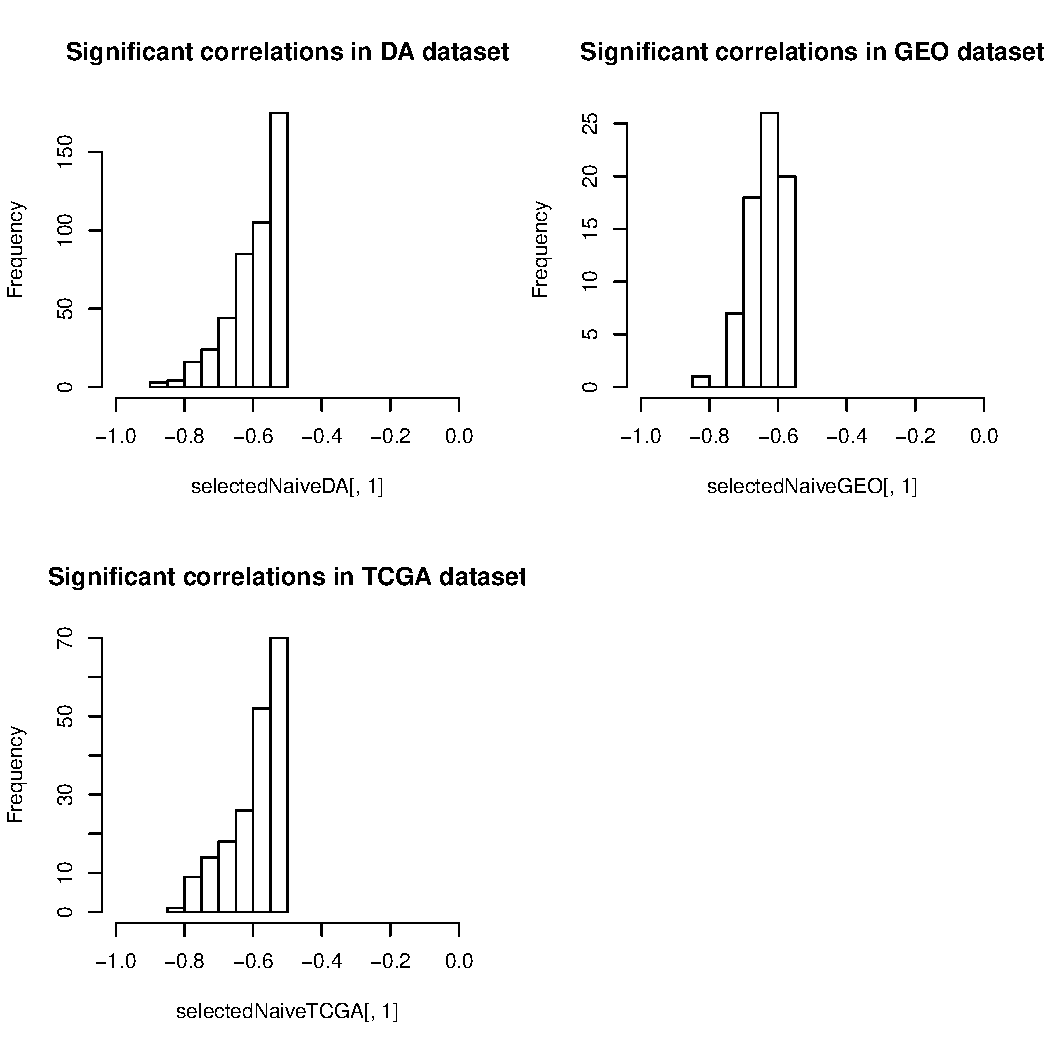
\includegraphics[width=\maxwidth]{figure/showCorrs-1} 

\end{knitrout}
\caption{Distribution of the correlation coefficients of the selected genes. Depending on the `pvalue` and the `r` cutoff more or less genes will be retained\label{showCorrs1}}
\end{figure}

The number of genes selected using the Naive method on the DA, TCGA and GEO datasets are respectively:
\begin{knitrout}
\definecolor{shadecolor}{rgb}{0.969, 0.969, 0.969}\color{fgcolor}\begin{kframe}
\begin{alltt}
\hlkwd{cat}\hlstd{(}\hlstr{"numNaive (DA): "}\hlstd{, numNaiveDA,}\hlstr{"\textbackslash{}n"}\hlstd{)}
\end{alltt}
\begin{verbatim}
## numNaive (DA):  456
\end{verbatim}
\begin{alltt}
\hlkwd{cat}\hlstd{(}\hlstr{"numNaive (GEO): "}\hlstd{, numNaiveGEO,}\hlstr{"\textbackslash{}n"}\hlstd{)}
\end{alltt}
\begin{verbatim}
## numNaive (GEO):  72
\end{verbatim}
\begin{alltt}
\hlkwd{cat}\hlstd{(}\hlstr{"numNaive (TCGA): "}\hlstd{, numNaiveTCGA,}\hlstr{"\textbackslash{}n"}\hlstd{)}
\end{alltt}
\begin{verbatim}
## numNaive (TCGA):  190
\end{verbatim}
\end{kframe}
\end{knitrout}

This can be visualized using Venn Diagrams:

\begin{knitrout}
\definecolor{shadecolor}{rgb}{0.969, 0.969, 0.969}\color{fgcolor}\begin{kframe}
\begin{alltt}
\hlstd{myVenn3}\hlkwb{<-} \hlkwd{venn.diagram}\hlstd{(}\hlkwc{x}\hlstd{=}\hlkwd{list}\hlstd{(}\hlkwc{naiveDA}\hlstd{=}\hlkwd{rownames}\hlstd{(selectedNaiveDA),}
                              \hlkwc{naiveGEO}\hlstd{=}\hlkwd{rownames}\hlstd{(selectedNaiveGEO),}
                              \hlkwc{naiveTCGA}\hlstd{=}\hlkwd{rownames}\hlstd{(selectedNaiveTCGA)),}
                              \hlkwc{filename}\hlstd{=}\hlkwa{NULL}\hlstd{,} \hlkwc{lty} \hlstd{=} \hlstr{"blank"}\hlstd{,}
                              \hlkwc{fill}\hlstd{=}\hlkwd{c}\hlstd{(}\hlstr{"pink1"}\hlstd{,} \hlstr{"skyblue"}\hlstd{,} \hlstr{"mediumorchid"}\hlstd{),}
                       \hlkwc{main}\hlstd{=}\hlstr{"Genes in common between the three -Naive selected- gene lists"}\hlstd{)}
\hlkwd{grid.newpage}\hlstd{()}
\hlkwd{grid.draw}\hlstd{(myVenn3)}
\end{alltt}
\end{kframe}
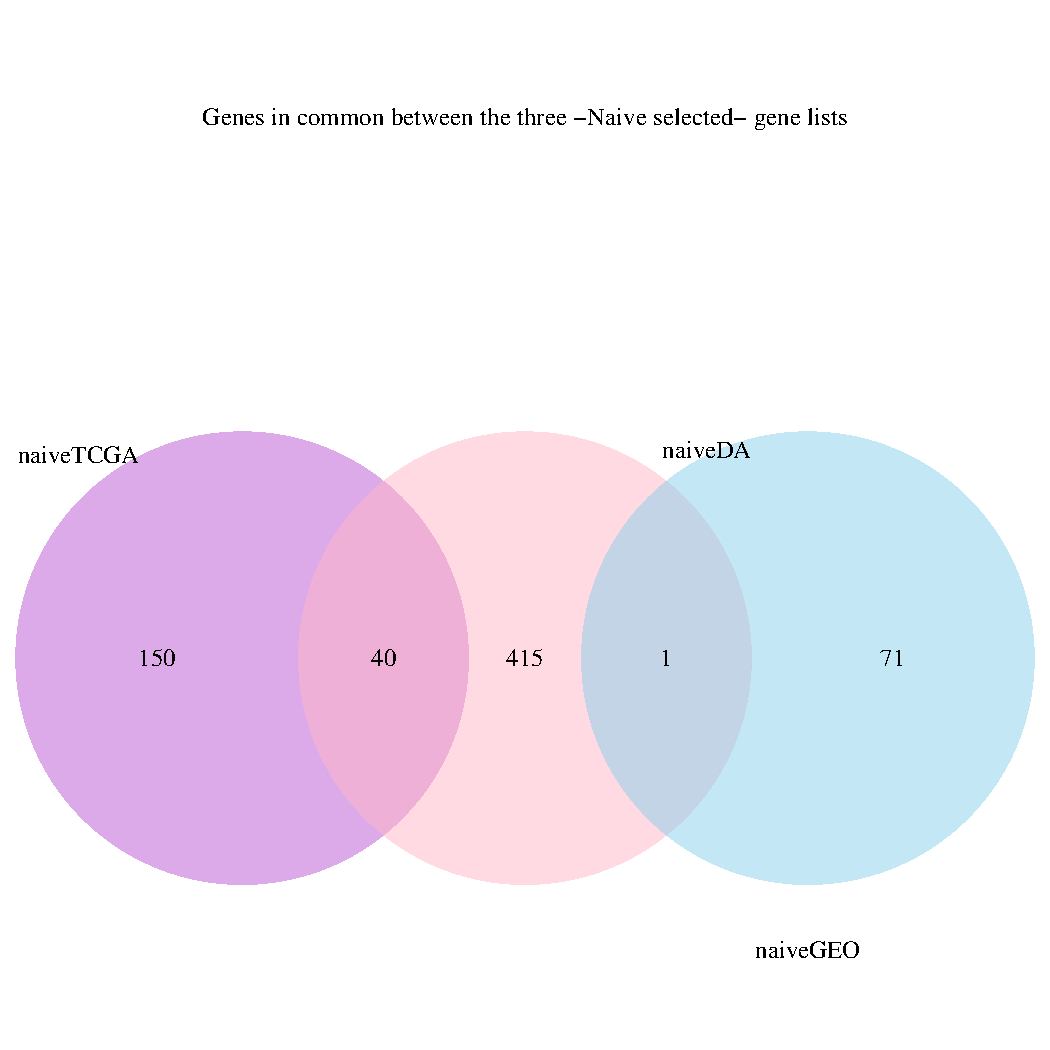
\includegraphics[width=\maxwidth]{figure/vennCommonGenesin3listsNaive-1} 

\end{knitrout}

\subsubsection{Naive selection on TRUE and FALSE candidates}

\begin{knitrout}
\definecolor{shadecolor}{rgb}{0.969, 0.969, 0.969}\color{fgcolor}\begin{kframe}
\begin{alltt}
\hlstd{naiveDATrueFalse} \hlkwb{<-} \hlkwd{naiveSelection} \hlstd{(}\hlkwd{as.matrix}\hlstd{(DATrueFalseExpr),} \hlkwd{as.matrix}\hlstd{(DATrueFalseMet),} \hlkwc{pValCutoff}\hlstd{=} \hlnum{0.25}\hlstd{,} \hlkwc{rCutoff}\hlstd{=}\hlnum{0}\hlstd{,} \hlkwc{type}\hlstd{=}\hlstr{"Spearman"}\hlstd{,} \hlkwc{adj}\hlstd{=}\hlnum{TRUE}\hlstd{)}
\hlstd{selectedNaiveDATrueFalse} \hlkwb{<-}\hlstd{naiveDATrueFalse[naiveDATrueFalse}\hlopt{$}\hlstd{SigNegCorr,]}
\hlstd{myVenn2}\hlkwb{<-} \hlkwd{venn.diagram}\hlstd{(}\hlkwc{x}\hlstd{=}\hlkwd{list}\hlstd{(}\hlkwc{naiveDATrueFalse}\hlstd{=}\hlkwd{rownames}\hlstd{(selectedNaiveDATrueFalse),} \hlkwc{TRUEL}\hlstd{=trueLGeneNames),} \hlkwc{filename}\hlstd{=}\hlkwa{NULL}\hlstd{,} \hlkwc{lty} \hlstd{=} \hlstr{"blank"}\hlstd{,}  \hlkwc{fill}\hlstd{=}\hlkwd{c}\hlstd{(}\hlstr{"pink1"}\hlstd{,} \hlstr{"skyblue"}\hlstd{),} \hlkwc{main}\hlstd{=}\hlstr{"Genes in common between TRUE L and -Naive selected from TRUE/FALSE- gene lists"}\hlstd{)}
\hlkwd{grid.newpage}\hlstd{()}
\hlkwd{grid.draw}\hlstd{(myVenn2)}
\end{alltt}
\end{kframe}
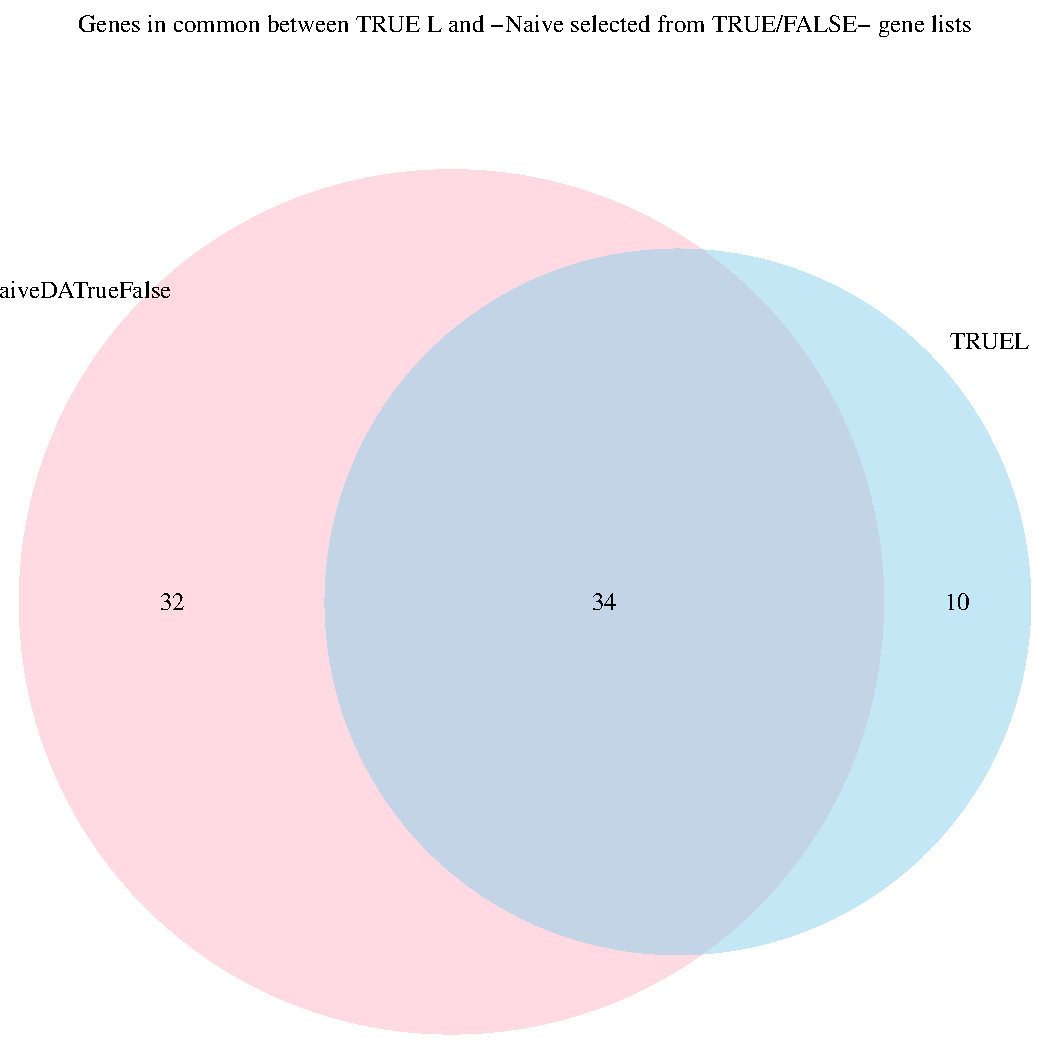
\includegraphics[width=\maxwidth]{figure/naiveSelTrueFalse-1} 
\begin{kframe}\begin{alltt}
\hlstd{myVenn2}\hlkwb{<-} \hlkwd{venn.diagram}\hlstd{(}\hlkwc{x}\hlstd{=}\hlkwd{list}\hlstd{(}\hlkwc{naiveDATrueFalse}\hlstd{=}\hlkwd{rownames}\hlstd{(selectedNaiveDATrueFalse),}
                              \hlkwc{FALSEL}\hlstd{=falseLGeneNames),}
                              \hlkwc{filename}\hlstd{=}\hlkwa{NULL}\hlstd{,} \hlkwc{lty} \hlstd{=} \hlstr{"blank"}\hlstd{,}
                              \hlkwc{fill}\hlstd{=}\hlkwd{c}\hlstd{(}\hlstr{"pink1"}\hlstd{,} \hlstr{"skyblue"}\hlstd{),}
                       \hlkwc{main}\hlstd{=}\hlstr{"Genes in common between FALSE L and -Naive selected from TRUE/FALSE- gene lists"}\hlstd{)}
\hlkwd{grid.newpage}\hlstd{()}
\hlkwd{grid.draw}\hlstd{(myVenn2)}
\end{alltt}
\end{kframe}
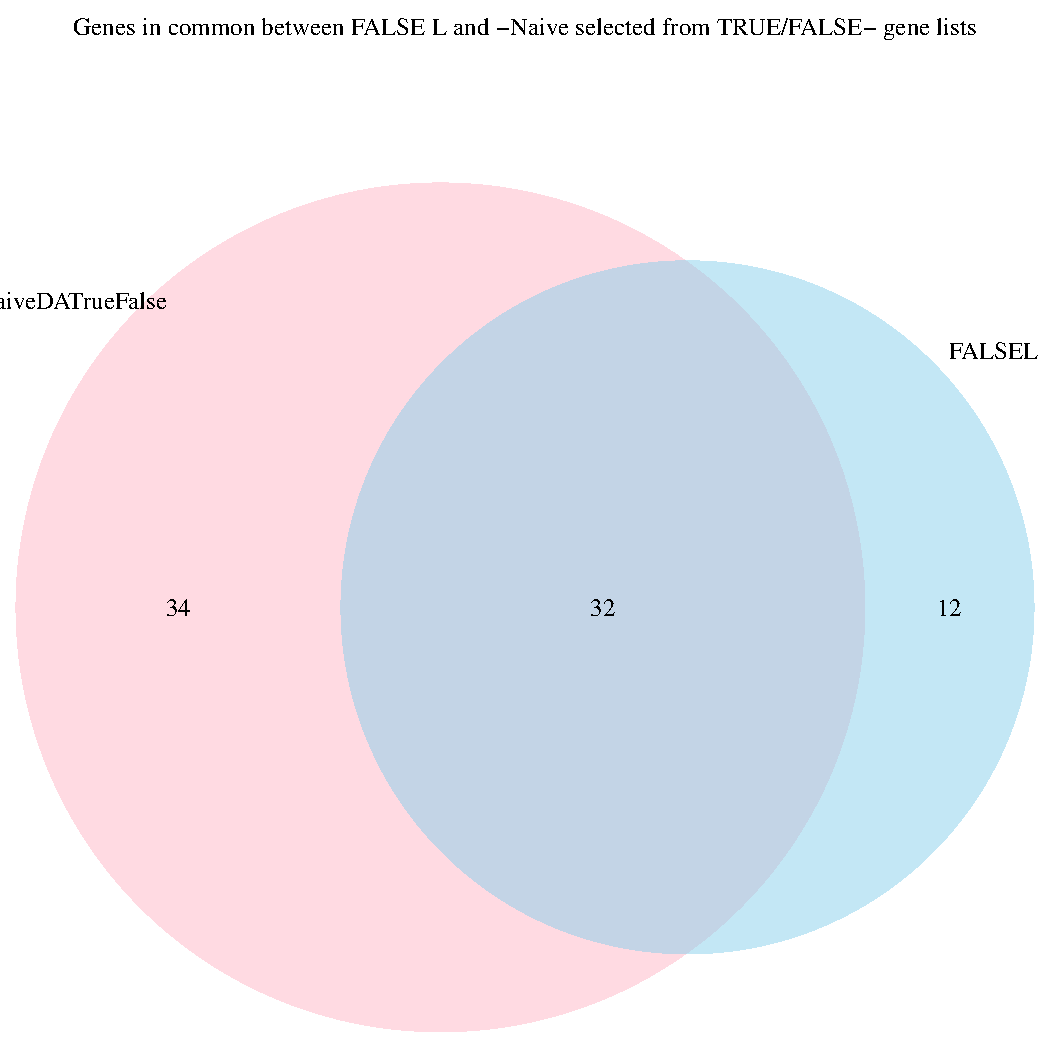
\includegraphics[width=\maxwidth]{figure/naiveSelTrueFalse-2} 

\end{knitrout}

\emph{It seems that both TRUE and FALSE L candidates are mostly negatively correlated}.


\subsection{Selecting L-shaped genes with the CMI method}

% As of 2017-08 the function for selecting genes based on CMI has experienced some problems so that instead of recomputing CMI based selection for all three gene sets we have recovered this gene list from a previous study

\begin{knitrout}
\definecolor{shadecolor}{rgb}{0.969, 0.969, 0.969}\color{fgcolor}\begin{kframe}
\begin{alltt}
\hlstd{calcAgainCMI} \hlkwb{<-} \hlnum{FALSE}
\hlkwa{if} \hlstd{(}\hlopt{!}\hlkwd{file.exists}\hlstd{(}\hlstr{"results/cmiSelections.Rda"}\hlstd{)} \hlopt{||} \hlstd{calcAgainCMI)\{}
  \hlkwd{system.time}\hlstd{(cmiDA} \hlkwb{<-} \hlkwd{cmiSelection} \hlstd{(}\hlkwc{methData} \hlstd{= DAMetilData,} \hlkwc{exprData} \hlstd{= DAExprData ))}
  \hlstd{selectedCmiDA} \hlkwb{<-}\hlstd{cmiDA[cmiDA[,}\hlstr{"meth_regulated"}\hlstd{],]}
  \hlkwd{system.time}\hlstd{(cmiGEO} \hlkwb{<-} \hlkwd{cmiSelection} \hlstd{(}\hlkwc{methData} \hlstd{= geoMetilData,} \hlkwc{exprData} \hlstd{= geoExprData))}
  \hlstd{selectedCmiGEO} \hlkwb{<-}\hlstd{cmiGEO[cmiGEO[,}\hlstr{"meth_regulated"}\hlstd{],]}
  \hlkwd{system.time}\hlstd{(cmiTCGA} \hlkwb{<-} \hlkwd{cmiSelection} \hlstd{(}\hlkwc{methData} \hlstd{= TCGAMetilData,} \hlkwc{exprData} \hlstd{= TCGAExprData))}
  \hlstd{selectedCmiTCGA} \hlkwb{<-}\hlstd{cmiTCGA[cmiTCGA[,}\hlstr{"meth_regulated"}\hlstd{],]}
  \hlkwd{save}\hlstd{(cmiDA, cmiGEO, cmiTCGA,}
         \hlstd{selectedCmiDA, selectedCmiGEO, selectedCmiTCGA,}
         \hlkwc{file}\hlstd{=}\hlstr{"results/cmiSelections.Rda"}\hlstd{)}
  \hlstd{selectedGenesCmiDA} \hlkwb{<-} \hlkwd{rownames}\hlstd{(selectedCmiDA)}
  \hlstd{selectedGenesCmiGEO} \hlkwb{<-} \hlkwd{rownames}\hlstd{(selectedCmiGEO)}
  \hlstd{selectedGenesCmiTCGA} \hlkwb{<-} \hlkwd{rownames}\hlstd{(selectedCmiTCGA)}
  \hlkwd{save}\hlstd{(selectedGenesCmiDA, selectedGenesCmiGEO, selectedGenesCmiTCGA,}
         \hlkwc{file}\hlstd{=}\hlstr{"results/cmiSelectionsGeneNames.Rda"}\hlstd{)}
\hlstd{\}}\hlkwa{else}\hlstd{\{}
    \hlkwd{load}\hlstd{(}\hlstr{"results/cmiSelections.Rda"}\hlstd{)}
    \hlkwd{load}\hlstd{(}\hlstr{"results/cmiSelectionsGeneNames.Rda"}\hlstd{)}
\hlstd{\}}
\end{alltt}
\end{kframe}
\end{knitrout}

The number of genes selected using the CMI method on the DA, TCGA and GEO datasets are respectively 
 795, 263 and 301.


This can be visualized using Venn Diagrams:

\begin{knitrout}
\definecolor{shadecolor}{rgb}{0.969, 0.969, 0.969}\color{fgcolor}\begin{kframe}
\begin{alltt}
\hlstd{myVenn3}\hlkwb{<-} \hlkwd{venn.diagram}\hlstd{(}\hlkwc{x}\hlstd{=}\hlkwd{list}\hlstd{(}\hlkwc{cmiDA}\hlstd{=}\hlkwd{rownames}\hlstd{(selectedCmiDA),}
                              \hlkwc{cmiGEO}\hlstd{=}\hlkwd{rownames}\hlstd{(selectedCmiGEO),}
                              \hlkwc{cmiTCGA}\hlstd{=}\hlkwd{rownames}\hlstd{(selectedCmiTCGA)),}
                              \hlkwc{filename}\hlstd{=}\hlkwa{NULL}\hlstd{,} \hlkwc{lty} \hlstd{=} \hlstr{"blank"}\hlstd{,}
                              \hlkwc{fill}\hlstd{=}\hlkwd{c}\hlstd{(}\hlstr{"pink1"}\hlstd{,} \hlstr{"skyblue"}\hlstd{,} \hlstr{"mediumorchid"}\hlstd{),}
                       \hlkwc{main}\hlstd{=}\hlstr{"Genes in common between the three -CMI selected- gene lists"}\hlstd{)}
\hlkwd{grid.newpage}\hlstd{()}
\hlkwd{grid.draw}\hlstd{(myVenn3)}
\end{alltt}
\end{kframe}
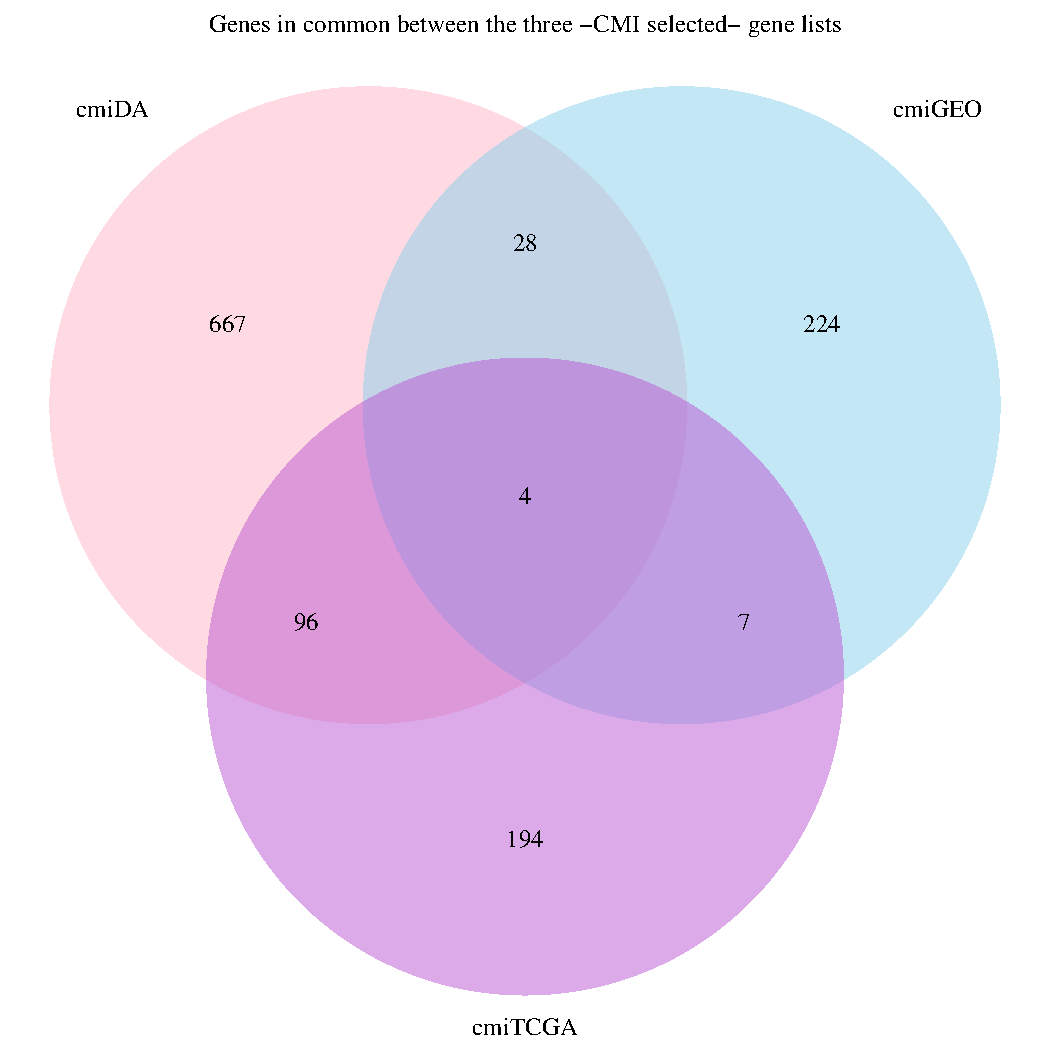
\includegraphics[width=\maxwidth]{figure/vennCommonGenesin3listsCMI-1} 

\end{knitrout}

\subsubsection{CMI selection on TRUE and FALSE candidates}

\begin{knitrout}
\definecolor{shadecolor}{rgb}{0.969, 0.969, 0.969}\color{fgcolor}\begin{kframe}
\begin{alltt}
\hlstd{cmiDATrueFalse} \hlkwb{<-} \hlkwd{cmiSelection} \hlstd{(DATrueFalseExpr, DATrueFalseMet)}
\hlstd{selectedCmiDATrueFalse} \hlkwb{<-}\hlstd{cmiDATrueFalse[cmiDATrueFalse[,}\hlstr{"meth_regulated"}\hlstd{],]}

\hlstd{myVenn2}\hlkwb{<-} \hlkwd{venn.diagram}\hlstd{(}\hlkwc{x}\hlstd{=}\hlkwd{list}\hlstd{(}\hlkwc{cmiDA}\hlstd{=}\hlkwd{rownames}\hlstd{(selectedCmiDA),}
                              \hlkwc{TRUEL}\hlstd{=trueLGeneNames),}
                              \hlkwc{filename}\hlstd{=}\hlkwa{NULL}\hlstd{,} \hlkwc{lty} \hlstd{=} \hlstr{"blank"}\hlstd{,}
                              \hlkwc{fill}\hlstd{=}\hlkwd{c}\hlstd{(}\hlstr{"pink1"}\hlstd{,} \hlstr{"skyblue"}\hlstd{),}
                       \hlkwc{main}\hlstd{=}\hlstr{"Genes in common between TRUE L and -CMI selected- gene lists"}\hlstd{)}
\hlkwd{grid.newpage}\hlstd{()}
\hlkwd{grid.draw}\hlstd{(myVenn2)}
\end{alltt}
\end{kframe}
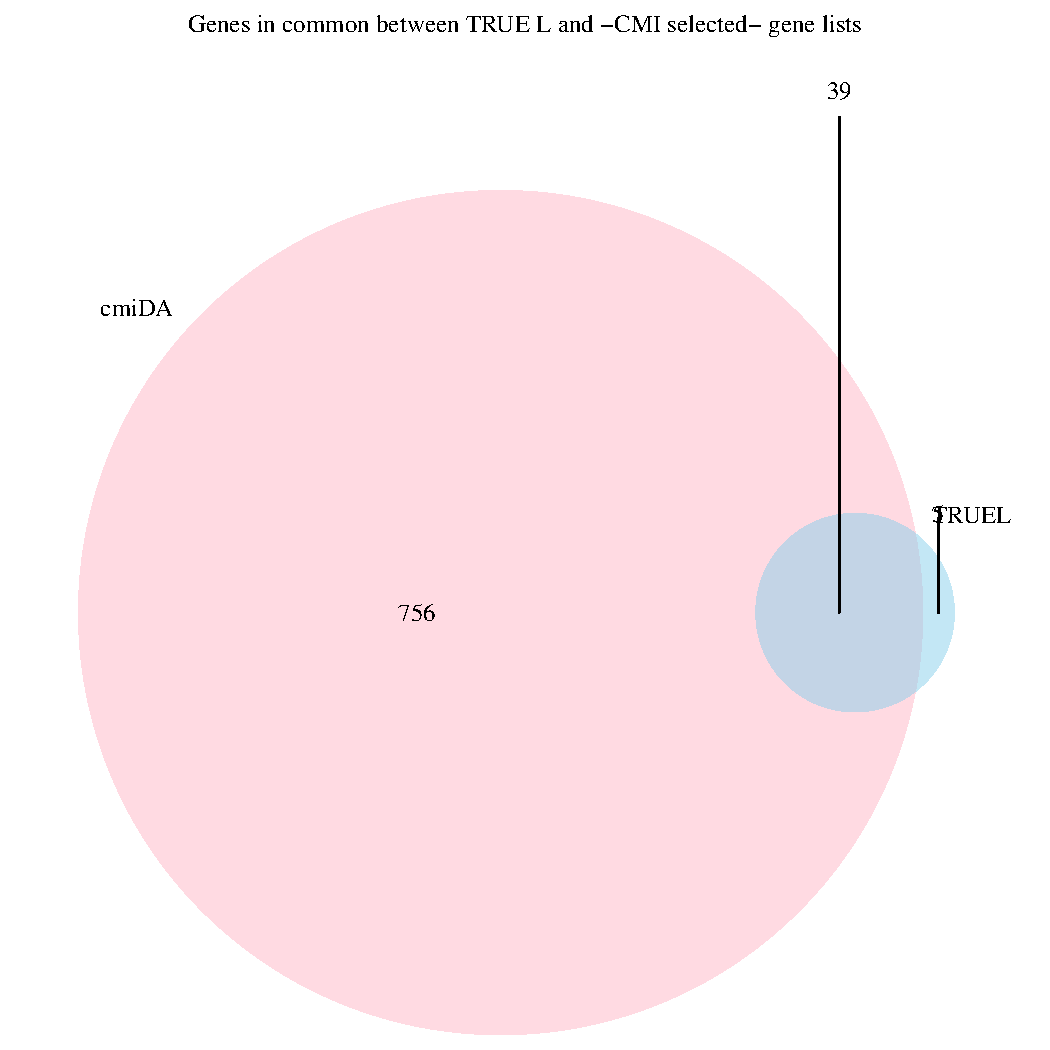
\includegraphics[width=\maxwidth]{figure/cmiSelTrue-1} 

\end{knitrout}

\begin{knitrout}
\definecolor{shadecolor}{rgb}{0.969, 0.969, 0.969}\color{fgcolor}\begin{kframe}
\begin{alltt}
\hlstd{myVenn2}\hlkwb{<-} \hlkwd{venn.diagram}\hlstd{(}\hlkwc{x}\hlstd{=}\hlkwd{list}\hlstd{(}\hlkwc{cmiDA}\hlstd{=}\hlkwd{rownames}\hlstd{(selectedCmiDA),}
                              \hlkwc{falseL}\hlstd{=falseLGeneNames),}
                              \hlkwc{filename}\hlstd{=}\hlkwa{NULL}\hlstd{,} \hlkwc{lty} \hlstd{=} \hlstr{"blank"}\hlstd{,}
                              \hlkwc{fill}\hlstd{=}\hlkwd{c}\hlstd{(}\hlstr{"pink1"}\hlstd{,} \hlstr{"skyblue"}\hlstd{),}
                       \hlkwc{main}\hlstd{=}\hlstr{"Genes in common between FALSE L and -CMI selected- gene lists"}\hlstd{)}
\hlkwd{grid.newpage}\hlstd{()}
\hlkwd{grid.draw}\hlstd{(myVenn2)}
\end{alltt}
\end{kframe}
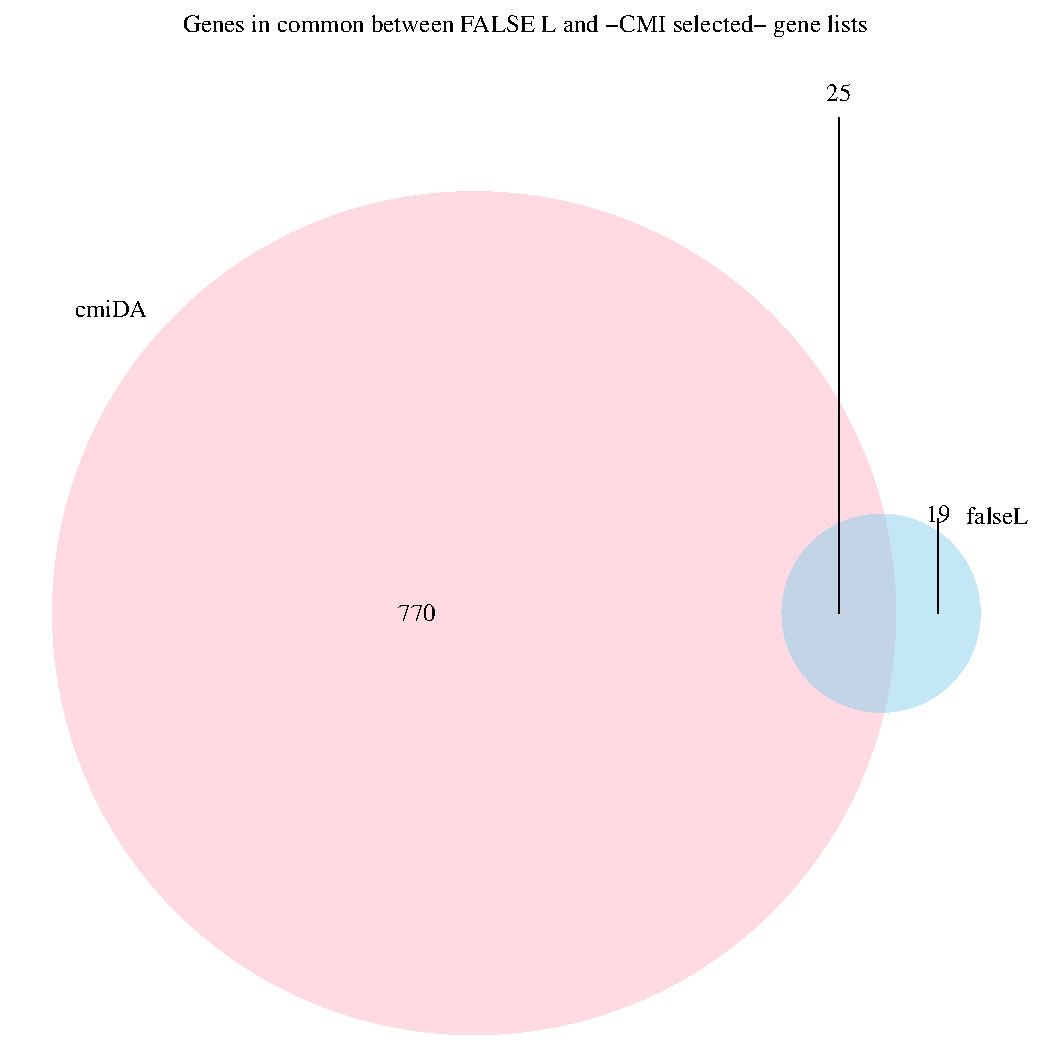
\includegraphics[width=\maxwidth]{figure/cmiSelFalse-1} 

\end{knitrout}

In this case it seems that the CMI method has selected more genes from the TRUE than from the FALSE example list.


\subsection{Selecting L-shaped genes with the \emph{heuristic} method}

The heuristic method is intended to select L-shaped scatterplots by overimposing a grid on it and defining certain regions which have to (or don't have to) contain a minimum (or maximum) percentage of points if the scatterplot is to be called L--shaped.

Besides this the method computes a scoring in such a way that scores in "good regions" score positively and points in "bad regions" score negatively. \emph{\textbf{An appropriate setting of scores and weights should yield positive scores for L-shaped scatterplots and negative scores for those that are not}}. 

One of the main interests of the approach presented here is the possibility to ``tune'' the selection process by changing the scoring parameters.

\begin{knitrout}
\definecolor{shadecolor}{rgb}{0.969, 0.969, 0.969}\color{fgcolor}\begin{kframe}
\begin{alltt}
\hlstd{(reqPercentages}   \hlkwb{<-} \hlkwd{matrix} \hlstd{(}\hlkwd{c}\hlstd{(}\hlnum{10}\hlstd{,} \hlnum{20}\hlstd{,} \hlnum{1}\hlstd{,} \hlnum{5}\hlstd{,} \hlnum{40}\hlstd{,} \hlnum{20}\hlstd{,} \hlnum{0}\hlstd{,} \hlnum{5}\hlstd{,} \hlnum{10}\hlstd{),} \hlkwc{nrow}\hlstd{=}\hlnum{3}\hlstd{,} \hlkwc{byrow}\hlstd{=}\hlnum{TRUE}\hlstd{))}
\end{alltt}
\end{kframe}


\begin{tabular}{r|r|r}
\hline
10 & 20 & 1\\
\hline
5 & 40 & 20\\
\hline
0 & 5 & 10\\
\hline
\end{tabular}\begin{kframe}\begin{alltt}
\hlstd{(maxminCounts} \hlkwb{<-} \hlkwd{toReqMat}\hlstd{(}\hlkwd{dim}\hlstd{(DAMetilData)[}\hlnum{2}\hlstd{], reqPercentages))} \hlcom{# Informative. NOt used in calculations because it is computed within the loop}
\end{alltt}
\end{kframe}


\begin{tabular}{r|r|r}
\hline
3 & 6 & 0\\
\hline
2 & 12 & 6\\
\hline
0 & 2 & 3\\
\hline
\end{tabular}\begin{kframe}\begin{alltt}
\hlstd{(reqPercentages4TCGA} \hlkwb{<-} \hlkwd{matrix} \hlstd{(}\hlkwd{c}\hlstd{(}\hlnum{4}\hlstd{,} \hlnum{20}\hlstd{,} \hlnum{5}\hlstd{,} \hlnum{1}\hlstd{,} \hlnum{40}\hlstd{,} \hlnum{20}\hlstd{,} \hlnum{0}\hlstd{,} \hlnum{1}\hlstd{,} \hlnum{4}\hlstd{),} \hlkwc{nrow}\hlstd{=}\hlnum{3}\hlstd{,} \hlkwc{byrow}\hlstd{=}\hlnum{TRUE}\hlstd{))}
\end{alltt}
\end{kframe}


\begin{tabular}{r|r|r}
\hline
4 & 20 & 5\\
\hline
1 & 40 & 20\\
\hline
0 & 1 & 4\\
\hline
\end{tabular}\begin{kframe}\begin{alltt}
\hlstd{(maxminCounts4TCGA} \hlkwb{<-} \hlkwd{toReqMat}\hlstd{(}\hlkwd{dim}\hlstd{(TCGAMetilData)[}\hlnum{2}\hlstd{], reqPercentages4TCGA))}
\end{alltt}
\end{kframe}


\begin{tabular}{r|r|r}
\hline
9 & 45 & 11\\
\hline
2 & 89 & 45\\
\hline
0 & 2 & 9\\
\hline
\end{tabular}\begin{kframe}\begin{alltt}
\hlstd{(theWeightMifL}\hlkwb{=}\hlkwd{matrix} \hlstd{(}\hlkwd{c}\hlstd{(}\hlnum{2}\hlstd{,}\hlopt{-}\hlnum{2}\hlstd{,}\hlopt{-}\hlnum{25}\hlstd{,}\hlnum{1}\hlstd{,}\hlnum{0}\hlstd{,}\hlopt{-}\hlnum{2}\hlstd{,}\hlnum{1}\hlstd{,}\hlnum{1}\hlstd{,}\hlnum{2}\hlstd{),} \hlkwc{nrow}\hlstd{=}\hlnum{3}\hlstd{,} \hlkwc{byrow}\hlstd{=}\hlnum{TRUE}\hlstd{))}
\end{alltt}
\end{kframe}


\begin{tabular}{r|r|r}
\hline
2 & -2 & -25\\
\hline
1 & 0 & -2\\
\hline
1 & 1 & 2\\
\hline
\end{tabular}\begin{kframe}\begin{alltt}
\hlstd{(theWeightMifNonL}\hlkwb{=}\hlkwd{matrix} \hlstd{(}\hlkwd{c}\hlstd{(}\hlnum{0}\hlstd{,}\hlopt{-}\hlnum{2}\hlstd{,}\hlopt{-}\hlnum{25}\hlstd{,}\hlnum{0}\hlstd{,}\hlnum{0}\hlstd{,}\hlopt{-}\hlnum{2}\hlstd{,}\hlnum{0}\hlstd{,}\hlnum{0}\hlstd{,}\hlnum{0}\hlstd{),} \hlkwc{nrow}\hlstd{=}\hlnum{3}\hlstd{,} \hlkwc{byrow}\hlstd{=}\hlnum{TRUE}\hlstd{))}
\end{alltt}
\end{kframe}


\begin{tabular}{r|r|r}
\hline
0 & -2 & -25\\
\hline
0 & 0 & -2\\
\hline
0 & 0 & 0\\
\hline
\end{tabular}
\end{knitrout}

\begin{knitrout}
\definecolor{shadecolor}{rgb}{0.969, 0.969, 0.969}\color{fgcolor}\begin{kframe}
\begin{alltt}
\hlstd{calcAgainHeuristic} \hlkwb{<-} \hlnum{TRUE} \hlcom{# Com donava error l'he calculat pas a pas i he gravat els resultats}
\hlkwa{if} \hlstd{(}\hlopt{!}\hlkwd{file.exists}\hlstd{(}\hlstr{"results/heuristicSelections.Rda"}\hlstd{)} \hlopt{||} \hlstd{calcAgainHeuristic)\{}
  \hlcom{# DA dataset}
  \hlstd{sampleSize} \hlkwb{<-} \hlkwd{dim}\hlstd{(DAMetilData)[}\hlnum{2}\hlstd{]}
  \hlstd{numGenes} \hlkwb{<-}   \hlkwd{dim}\hlstd{(DAMetilData)[}\hlnum{1}\hlstd{]}

  \hlkwd{messageTitle}\hlstd{(}\hlstr{"Scoring ALL genes in the DA (microarrays) dataset"}\hlstd{)}

  \hlstd{scoresDA1} \hlkwb{<-} \hlkwd{scoreGenesMat} \hlstd{(}\hlkwc{mets}\hlstd{=DAMetilData,}
                                                                      \hlkwc{expres}\hlstd{=DAExprData,}
                            \hlkwc{aReqPercentsMat}\hlstd{=reqPercentages,}
                            \hlkwc{aWeightMifL}\hlstd{=theWeightMifL,}
                            \hlkwc{aWeightMifNonL}\hlstd{=theWeightMifNonL )}
  \hlkwd{cat}\hlstd{(}\hlstr{"Number of scatterplots scored  : "}\hlstd{,} \hlkwd{dim}\hlstd{(scoresDA1)[}\hlnum{1}\hlstd{],}\hlstr{"\textbackslash{}n"}\hlstd{)}
  \hlkwd{cat}\hlstd{(}\hlstr{"Number of L-shape scatterplots : "}\hlstd{,} \hlkwd{sum}\hlstd{(scoresDA1[,}\hlnum{1}\hlstd{]),}\hlstr{"\textbackslash{}n"}\hlstd{)}
  \hlkwd{head}\hlstd{(scoresDA1)}
  \hlkwd{table}\hlstd{(scoresDA1[,}\hlnum{1}\hlstd{])}
  \hlstd{selectedHeuristicDA} \hlkwb{<-} \hlstd{scoresDA1[scoresDA1}\hlopt{$}\hlstd{logicSc,]}

  \hlcom{#GEO dataset}
  \hlkwd{messageTitle}\hlstd{(}\hlstr{"Scoring ALL genes in the GEO dataset"}\hlstd{)}
  \hlstd{sampleSize} \hlkwb{<-} \hlkwd{dim}\hlstd{(geoMetilData)[}\hlnum{2}\hlstd{]}
  \hlstd{scoresGEO} \hlkwb{<-} \hlkwd{scoreGenesMat} \hlstd{(}\hlkwc{mets}\hlstd{=geoMetilData,}
                            \hlkwc{expres}\hlstd{=geoExprData,}
                            \hlkwc{aReqPercentsMat}\hlstd{=reqPercentages,}
                            \hlkwc{aWeightMifL}\hlstd{=theWeightMifL,}
                            \hlkwc{aWeightMifNonL}\hlstd{=theWeightMifNonL )}
  \hlkwd{cat}\hlstd{(}\hlstr{"Number of scatterplots scored  : "}\hlstd{,} \hlkwd{dim}\hlstd{(scoresGEO)[}\hlnum{1}\hlstd{],} \hlstr{"\textbackslash{}n"}\hlstd{)}
  \hlkwd{cat}\hlstd{(}\hlstr{"Number of L-shape scatterplots : "}\hlstd{,} \hlkwd{sum}\hlstd{(scoresGEO[,}\hlnum{1}\hlstd{]),} \hlstr{"\textbackslash{}n"}\hlstd{)}
  \hlkwd{table}\hlstd{(scoresGEO[,}\hlnum{1}\hlstd{])}
  \hlstd{selectedHeuristicGEO} \hlkwb{<-} \hlstd{scoresGEO[scoresGEO}\hlopt{$}\hlstd{logicSc,]}

  \hlcom{#TCGA dataset}
  \hlstd{(numGenes} \hlkwb{<-}   \hlkwd{dim}\hlstd{(TCGAMetilData)[}\hlnum{1}\hlstd{])}
  \hlstd{(sampleSize} \hlkwb{<-} \hlkwd{dim}\hlstd{(TCGAMetilData)[}\hlnum{2}\hlstd{])}

  \hlstd{reqPercentages} \hlkwb{<-} \hlkwd{matrix} \hlstd{(}\hlkwd{c}\hlstd{(}\hlnum{2}\hlstd{,} \hlnum{20}\hlstd{,} \hlnum{5}\hlstd{,} \hlnum{1}\hlstd{,} \hlnum{40}\hlstd{,} \hlnum{20}\hlstd{,} \hlnum{0}\hlstd{,} \hlnum{1}\hlstd{,} \hlnum{2}\hlstd{),} \hlkwc{nrow}\hlstd{=}\hlnum{3}\hlstd{,} \hlkwc{byrow}\hlstd{=}\hlnum{TRUE}\hlstd{)}
  \hlstd{(maxminCounts} \hlkwb{<-} \hlkwd{toReqMat}\hlstd{(sampleSize, reqPercentages))}

  \hlstd{(theWeightMifL}\hlkwb{=}\hlkwd{matrix} \hlstd{(}\hlkwd{c}\hlstd{(}\hlnum{2}\hlstd{,}\hlopt{-}\hlnum{2}\hlstd{,}\hlopt{-}\hlstd{sampleSize}\hlopt{/}\hlnum{5}\hlstd{,}\hlnum{1}\hlstd{,}\hlnum{0}\hlstd{,}\hlopt{-}\hlnum{2}\hlstd{,}\hlnum{1}\hlstd{,}\hlnum{1}\hlstd{,}\hlnum{2}\hlstd{),} \hlkwc{nrow}\hlstd{=}\hlnum{3}\hlstd{,} \hlkwc{byrow}\hlstd{=}\hlnum{TRUE}\hlstd{))}
  \hlstd{(theWeightMifNonL}\hlkwb{=}\hlkwd{matrix} \hlstd{(}\hlkwd{c}\hlstd{(}\hlnum{0}\hlstd{,}\hlopt{-}\hlnum{2}\hlstd{,}\hlopt{-}\hlstd{sampleSize}\hlopt{/}\hlnum{5}\hlstd{,}\hlnum{0}\hlstd{,}\hlnum{0}\hlstd{,}\hlopt{-}\hlnum{2}\hlstd{,}\hlnum{0}\hlstd{,}\hlnum{0}\hlstd{,}\hlnum{0}\hlstd{),} \hlkwc{nrow}\hlstd{=}\hlnum{3}\hlstd{,} \hlkwc{byrow}\hlstd{=}\hlnum{TRUE}\hlstd{))}

  \hlkwd{messageTitle}\hlstd{(}\hlstr{"Scoring ALL genes in the TCGA (microarrays) dataset"}\hlstd{)}
  \hlstd{scoresTCGA} \hlkwb{<-} \hlkwd{scoreGenesMat} \hlstd{(}\hlkwc{mets}\hlstd{=TCGAMetilData,}
                                                                      \hlkwc{expres}\hlstd{=TCGAExprData,}
                                                                       \hlkwc{x1}\hlstd{=}\hlnum{1}\hlopt{/}\hlnum{3}\hlstd{,} \hlkwc{x2}\hlstd{=}\hlnum{2}\hlopt{/}\hlnum{3}\hlstd{,}
                            \hlkwc{aReqPercentsMat}\hlstd{=reqPercentages,}
                            \hlkwc{aWeightMifL}\hlstd{=theWeightMifL,}
                            \hlkwc{aWeightMifNonL}\hlstd{=theWeightMifNonL )}
  \hlkwd{cat}\hlstd{(}\hlstr{"Number of scatterplots scored  : "}\hlstd{,} \hlkwd{dim}\hlstd{(scoresTCGA)[}\hlnum{1}\hlstd{],}\hlstr{"\textbackslash{}n"}\hlstd{)}
  \hlkwd{cat}\hlstd{(}\hlstr{"Number of L-shape scatterplots : "}\hlstd{,} \hlkwd{sum}\hlstd{(scoresTCGA[,}\hlnum{1}\hlstd{]),}\hlstr{"\textbackslash{}n"}\hlstd{)}
  \hlkwd{head}\hlstd{(scoresTCGA)}
  \hlkwd{table}\hlstd{(scoresTCGA[,}\hlnum{1}\hlstd{])}
  \hlstd{selectedHeuristicTCGA} \hlkwb{<-} \hlstd{scoresTCGA[scoresTCGA}\hlopt{$}\hlstd{logicSc,]}

  \hlkwd{save}\hlstd{(scoresDA1, scoresGEO, scoresTCGA,}
       \hlstd{selectedHeuristicDA, selectedHeuristicGEO, selectedHeuristicTCGA,}
         \hlkwc{file}\hlstd{=}\hlstr{"results/heuristicSelections.Rda"}\hlstd{)}
  \hlstd{selectedGenesHeuristicDA} \hlkwb{<-} \hlkwd{rownames}\hlstd{(selectedHeuristicDA)}
  \hlstd{selectedGenesHeuristicGEO} \hlkwb{<-} \hlkwd{rownames}\hlstd{(selectedHeuristicGEO)}
  \hlstd{selectedGenesHeuristicTCGA} \hlkwb{<-} \hlkwd{rownames}\hlstd{(selectedHeuristicTCGA)}
  \hlkwd{save}\hlstd{(selectedGenesHeuristicDA,selectedGenesHeuristicGEO, selectedGenesHeuristicTCGA,} \hlkwc{file}\hlstd{=}\hlstr{"results/heuristicSelectionsGeneNames.Rda"}\hlstd{)}
\hlstd{\}}\hlkwa{else}\hlstd{\{}
    \hlkwd{load}\hlstd{(}\hlstr{"results/heuristicSelections.Rda"}\hlstd{)}
   \hlkwd{load}\hlstd{(}\hlstr{"results/heuristicSelectionsGeneNames.Rda"}\hlstd{)}
\hlstd{\}}
\end{alltt}
\begin{verbatim}
## Scoring ALL genes in the DA (microarrays) dataset 
## ------------------------------------------------- 
## Number of scatterplots scored  :  11359 
## Number of L-shape scatterplots :  188 
## Scoring ALL genes in the GEO dataset 
## ------------------------------------ 
## Number of scatterplots scored  :  11191 
## Number of L-shape scatterplots :  39 
## Scoring ALL genes in the TCGA (microarrays) dataset 
## --------------------------------------------------- 
## Number of scatterplots scored  :  11788 
## Number of L-shape scatterplots :  735
\end{verbatim}
\end{kframe}
\end{knitrout}


We may select L genes and plot only these.
The resulting plots are available in files 
\begin{itemize}
  \item \texttt{DAExprLGenesScores.pdf}
  \item \texttt{GEOLGenesScores.pdf}
  \item \texttt{TCGALGenesScores.pdf}
\end{itemize}

\begin{knitrout}
\definecolor{shadecolor}{rgb}{0.969, 0.969, 0.969}\color{fgcolor}\begin{kframe}
\begin{alltt}
\hlstd{LgenesDAExpr} \hlkwb{<-} \hlstd{DAExprData[scoresDA1[,}\hlstr{"logicSc"}\hlstd{],]}
\hlkwd{dim}\hlstd{(LgenesDAExpr)}
\end{alltt}
\begin{verbatim}
## [1] 188  30
\end{verbatim}
\begin{alltt}
\hlstd{geneListLDAExpr} \hlkwb{<-} \hlkwd{rownames}\hlstd{(DAExprData[scoresDA1[,}\hlstr{"logicSc"}\hlstd{],])}
\hlkwd{plotGenesMat} \hlstd{(}\hlkwc{mets}\hlstd{=DAMetilData[geneListLDAExpr,],}
              \hlkwc{expres}\hlstd{=DAExprData[geneListLDAExpr,],}
              \hlkwc{fileName} \hlstd{=}\hlstr{"results/DAExprLGenesScores.pdf"}\hlstd{,}
              \hlkwc{text4Title} \hlstd{= scoresDA1[geneListLDAExpr,}\hlstr{"numericSc"}\hlstd{])}
\end{alltt}
\begin{verbatim}
## pdf 
##   2
\end{verbatim}
\begin{alltt}
\hlstd{LgenesGEOExpr} \hlkwb{<-} \hlstd{geoExprData[scoresGEO[,}\hlstr{"logicSc"}\hlstd{],]}
\hlkwd{dim}\hlstd{(LgenesGEOExpr)}
\end{alltt}
\begin{verbatim}
## [1] 39 25
\end{verbatim}
\begin{alltt}
\hlstd{geneListLGEOExpr} \hlkwb{<-} \hlkwd{rownames}\hlstd{(geoExprData[scoresGEO[,}\hlstr{"logicSc"}\hlstd{],])}
\hlkwd{plotGenesMat} \hlstd{(}\hlkwc{mets}\hlstd{=geoMetilData[geneListLGEOExpr,],}
              \hlkwc{expres}\hlstd{=geoExprData[geneListLGEOExpr,],}
              \hlkwc{fileName} \hlstd{=}\hlstr{"results/geoExprLGenesScores.pdf"}\hlstd{,}
              \hlkwc{text4Title} \hlstd{= scoresGEO[geneListLGEOExpr,}\hlstr{"numericSc"}\hlstd{])}
\end{alltt}
\begin{verbatim}
## pdf 
##   2
\end{verbatim}
\begin{alltt}
\hlstd{myVenn2}\hlkwb{<-} \hlkwd{venn.diagram}\hlstd{(}\hlkwc{x}\hlstd{=}\hlkwd{list}\hlstd{(}\hlkwc{DAMicroarrays}\hlstd{=geneListLDAExpr,}
                              \hlkwc{GEO}\hlstd{=geneListLGEOExpr),}
                              \hlkwc{filename}\hlstd{=}\hlkwa{NULL}\hlstd{,} \hlkwc{lty} \hlstd{=} \hlstr{"blank"}\hlstd{,}
                              \hlkwc{fill}\hlstd{=}\hlkwd{c}\hlstd{(}\hlstr{"pink1"}\hlstd{,} \hlstr{"skyblue"}\hlstd{))}
\hlkwd{grid.newpage}\hlstd{()}
\hlkwd{grid.draw}\hlstd{(myVenn2)}
\end{alltt}
\end{kframe}
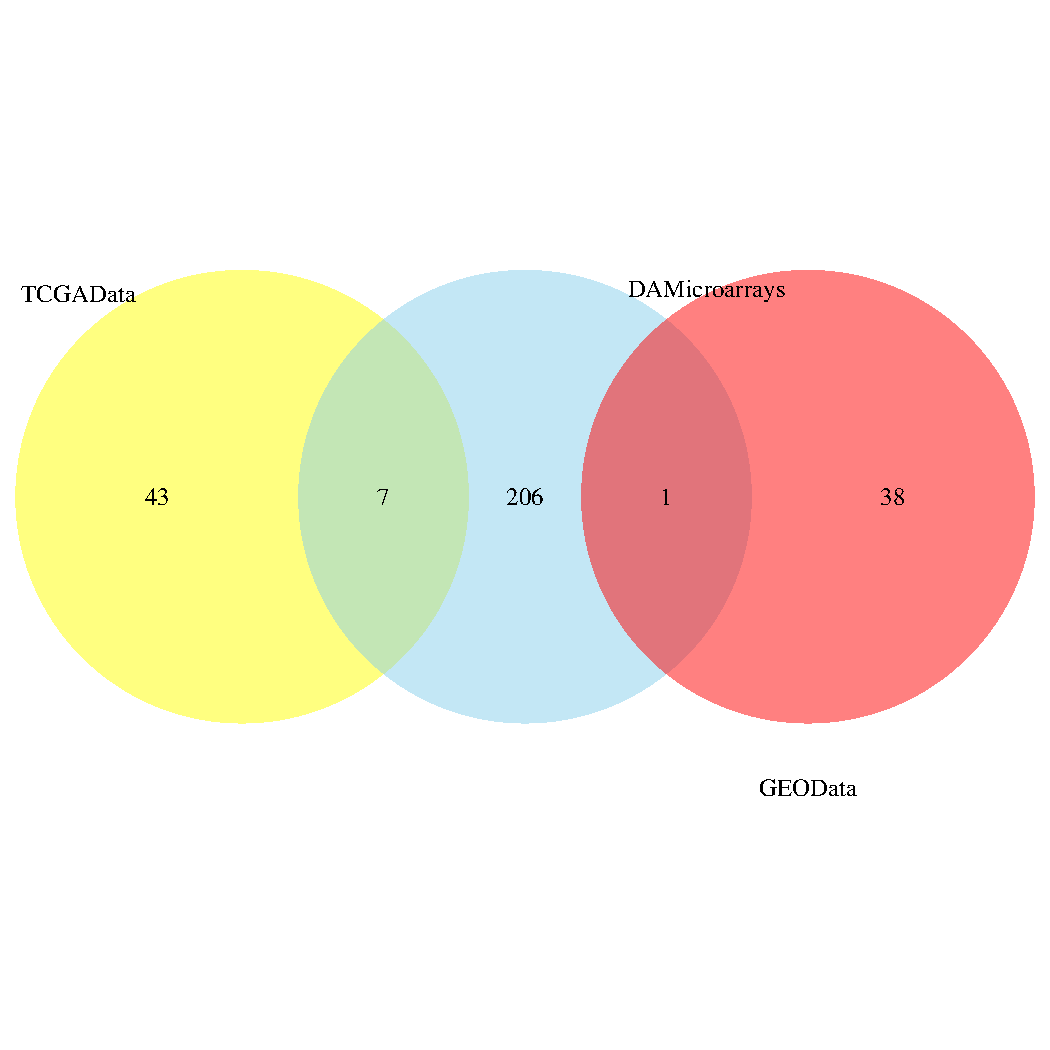
\includegraphics[width=\maxwidth]{figure/selectLGenes1-1} 
\begin{kframe}\begin{alltt}
\hlstd{LgenesTCGAExpr} \hlkwb{<-} \hlstd{TCGAExprData[scoresTCGA}\hlopt{$}\hlstd{numericSc} \hlopt{>}\hlnum{100}\hlstd{, ]}
\hlkwd{dim}\hlstd{(LgenesTCGAExpr)}
\end{alltt}
\begin{verbatim}
## [1] 442 223
\end{verbatim}
\begin{alltt}
\hlstd{geneListLTCGAExpr} \hlkwb{<-} \hlkwd{rownames}\hlstd{(TCGAExprData[scoresTCGA}\hlopt{$}\hlstd{numericSc} \hlopt{>}\hlnum{100}\hlstd{, ])}


\hlstd{myVenn3}\hlkwb{<-} \hlkwd{venn.diagram}\hlstd{(}\hlkwc{x}\hlstd{=}\hlkwd{list}\hlstd{(}\hlkwc{DAMicroarrays}\hlstd{=geneListLDAExpr,}
                              \hlkwc{TCGA}\hlstd{=geneListLTCGAExpr),}
                              \hlkwc{filename}\hlstd{=}\hlkwa{NULL}\hlstd{,} \hlkwc{lty} \hlstd{=} \hlstr{"blank"}\hlstd{,}
                              \hlkwc{fill}\hlstd{=}\hlkwd{c}\hlstd{(}\hlstr{"pink1"}\hlstd{,} \hlstr{"skyblue"}\hlstd{))}
\hlkwd{grid.newpage}\hlstd{()}
\hlkwd{grid.draw}\hlstd{(myVenn3)}
\end{alltt}
\end{kframe}
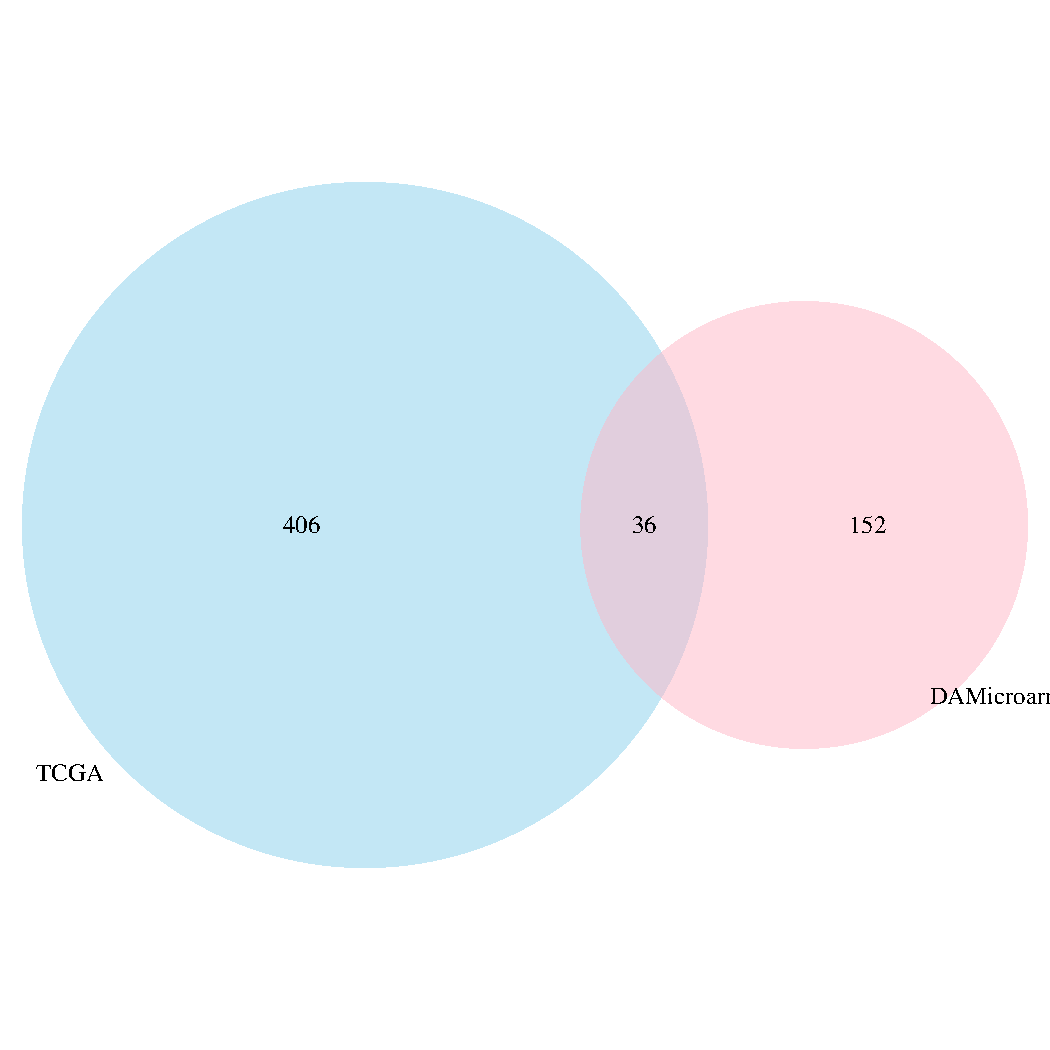
\includegraphics[width=\maxwidth]{figure/selectLGenes1-2} 

\end{knitrout}

\begin{knitrout}
\definecolor{shadecolor}{rgb}{0.969, 0.969, 0.969}\color{fgcolor}\begin{kframe}
\begin{alltt}
\hlstd{myVenn4H}\hlkwb{<-} \hlkwd{venn.diagram}\hlstd{(}\hlkwc{x}\hlstd{=}\hlkwd{list}\hlstd{(}\hlkwc{DAMicroarrays}\hlstd{=geneListLDAExpr,}
                              \hlkwc{GEO}\hlstd{=geneListLGEOExpr,}
                              \hlkwc{TCGA}\hlstd{=geneListLTCGAExpr),}
                              \hlkwc{filename}\hlstd{=}\hlkwa{NULL}\hlstd{,} \hlkwc{lty} \hlstd{=} \hlstr{"blank"}\hlstd{,}
                              \hlkwc{fill}\hlstd{=}\hlkwd{c}\hlstd{(}\hlstr{"pink1"}\hlstd{,} \hlstr{"skyblue"}\hlstd{,} \hlstr{"mediumorchid"}\hlstd{),}
                           \hlkwc{main}\hlstd{=}\hlstr{"Genes in common between the three -heuristic selected- gene lists"}\hlstd{)}
\hlkwd{grid.newpage}\hlstd{()}
\hlkwd{grid.draw}\hlstd{(myVenn4H)}
\end{alltt}
\end{kframe}
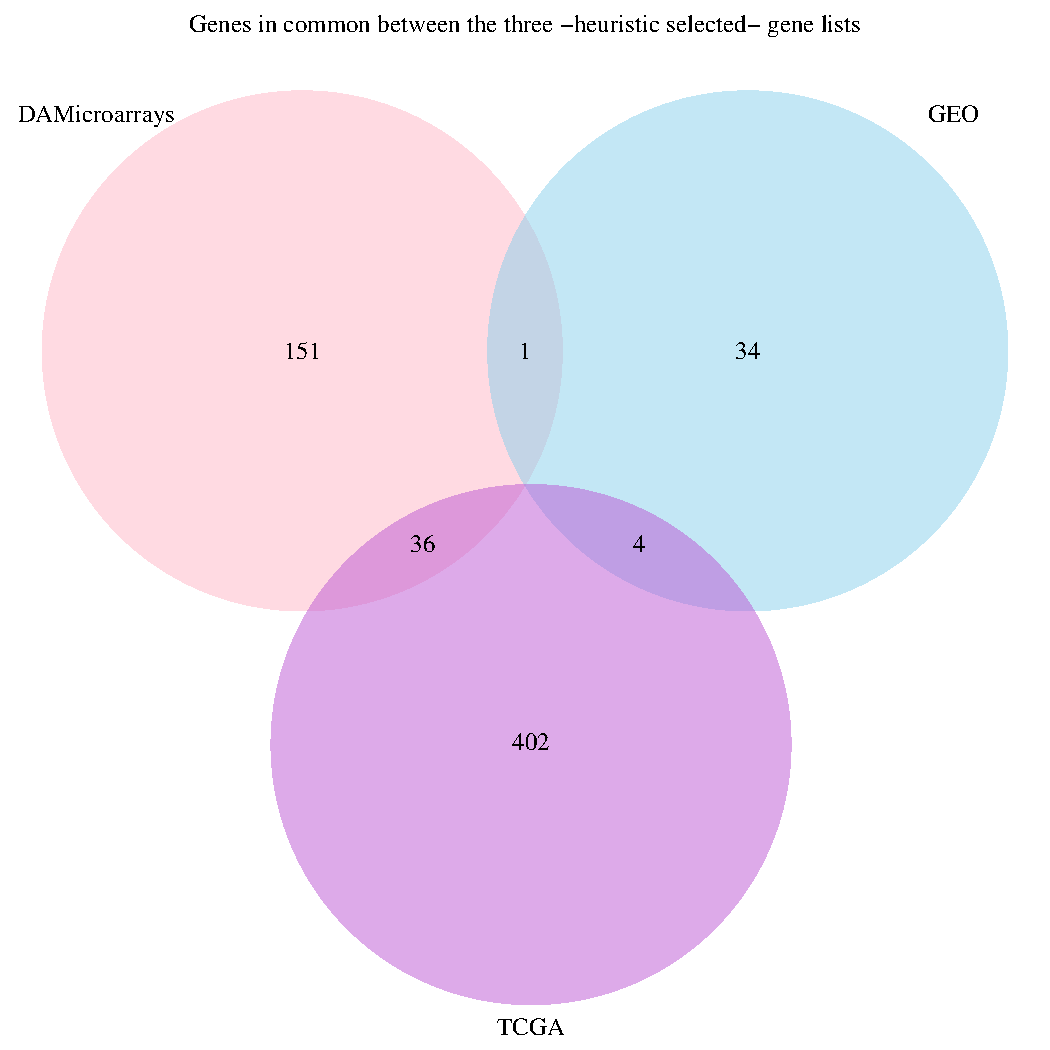
\includegraphics[width=\maxwidth]{figure/commonHeuristic3-1} 

\end{knitrout}


\section{Comparison between the selected lists}

What is the level of concordance between the three methods? This obviously may depend on the parameters of each method but for the values set her we obtain the following coincidences.

\begin{knitrout}
\definecolor{shadecolor}{rgb}{0.969, 0.969, 0.969}\color{fgcolor}\begin{kframe}
\begin{alltt}
\hlstd{myVenn3DA}\hlkwb{<-} \hlkwd{venn.diagram}\hlstd{(}\hlkwc{x}\hlstd{=}\hlkwd{list}\hlstd{(}\hlkwc{naiveDA}\hlstd{=}\hlkwd{rownames}\hlstd{(selectedNaiveDA),}
                                \hlkwc{cmiDA}\hlstd{=}\hlkwd{rownames}\hlstd{(selectedCmiDA),}
                                \hlkwc{heuristicDA} \hlstd{=} \hlkwd{rownames}\hlstd{(selectedHeuristicDA)),}
                                \hlkwc{filename}\hlstd{=}\hlkwa{NULL}\hlstd{,} \hlkwc{lty} \hlstd{=} \hlstr{"blank"}\hlstd{,}
                                \hlkwc{fill}\hlstd{=}\hlkwd{c}\hlstd{(}\hlstr{"pink1"}\hlstd{,} \hlstr{"skyblue"}\hlstd{,} \hlstr{"mediumorchid"}\hlstd{),}
                       \hlkwc{main}\hlstd{=}\hlstr{"Genes in common between the 3 methods in DA dataset"}\hlstd{)}
\hlkwd{grid.newpage}\hlstd{()}
\hlkwd{grid.draw}\hlstd{(myVenn3DA)}
\end{alltt}
\end{kframe}
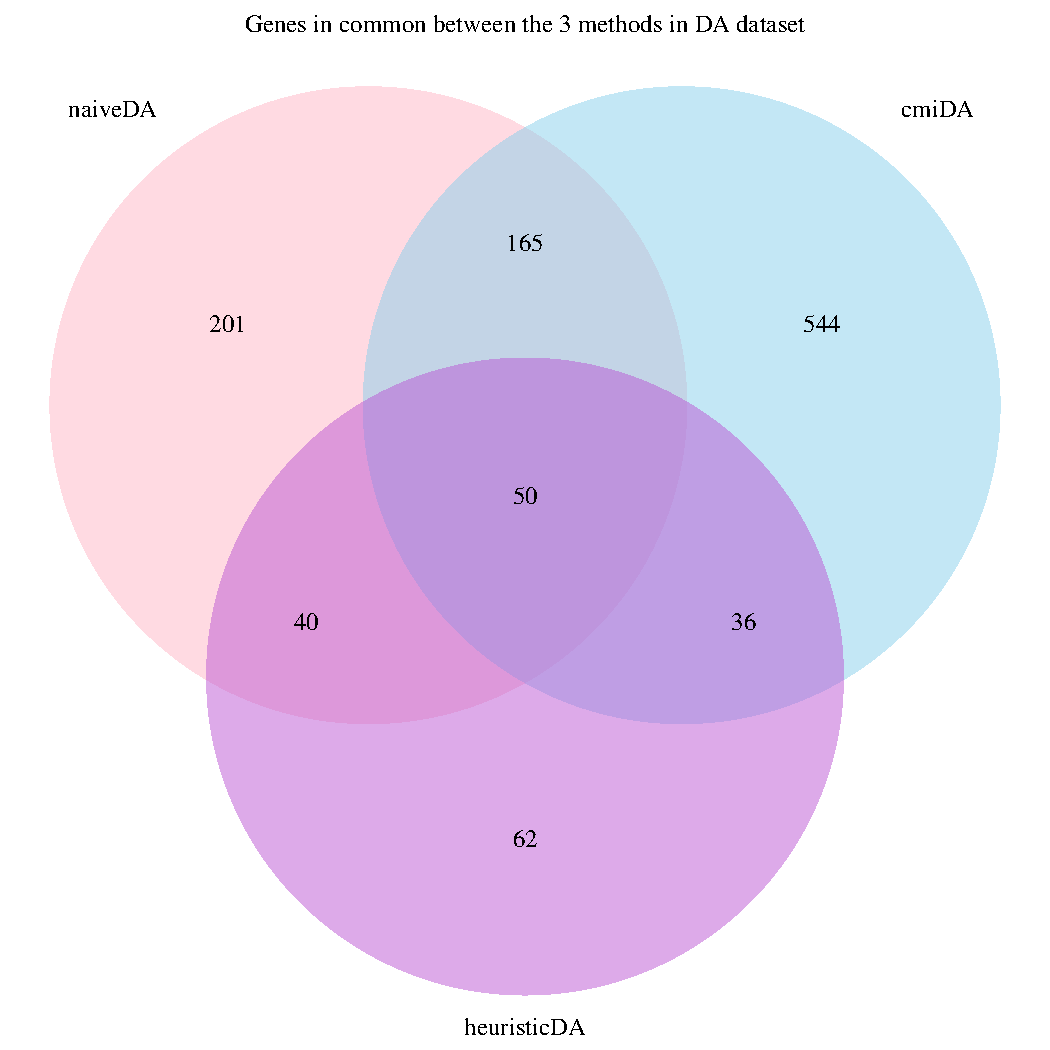
\includegraphics[width=\maxwidth]{figure/compare3DA-1} 

\end{knitrout}

\begin{knitrout}
\definecolor{shadecolor}{rgb}{0.969, 0.969, 0.969}\color{fgcolor}\begin{kframe}
\begin{alltt}
\hlstd{myVenn3GEO}\hlkwb{<-} \hlkwd{venn.diagram}\hlstd{(}\hlkwc{x}\hlstd{=}\hlkwd{list}\hlstd{(}\hlkwc{naiveGEO}\hlstd{=}\hlkwd{rownames}\hlstd{(selectedNaiveGEO),}
                                \hlkwc{cmiGEO}\hlstd{=}\hlkwd{rownames}\hlstd{(selectedCmiGEO),}
                                \hlkwc{heuristicGEO} \hlstd{=} \hlkwd{rownames}\hlstd{(selectedHeuristicGEO)),}
                                \hlkwc{filename}\hlstd{=}\hlkwa{NULL}\hlstd{,} \hlkwc{lty} \hlstd{=} \hlstr{"blank"}\hlstd{,}
                                \hlkwc{fill}\hlstd{=}\hlkwd{c}\hlstd{(}\hlstr{"pink1"}\hlstd{,} \hlstr{"skyblue"}\hlstd{,} \hlstr{"mediumorchid"}\hlstd{),}
                       \hlkwc{main}\hlstd{=}\hlstr{"Genes in common between the 3 methods in GEO dataset"}\hlstd{)}
\hlkwd{grid.newpage}\hlstd{()}
\hlkwd{grid.draw}\hlstd{(myVenn3GEO)}
\end{alltt}
\end{kframe}
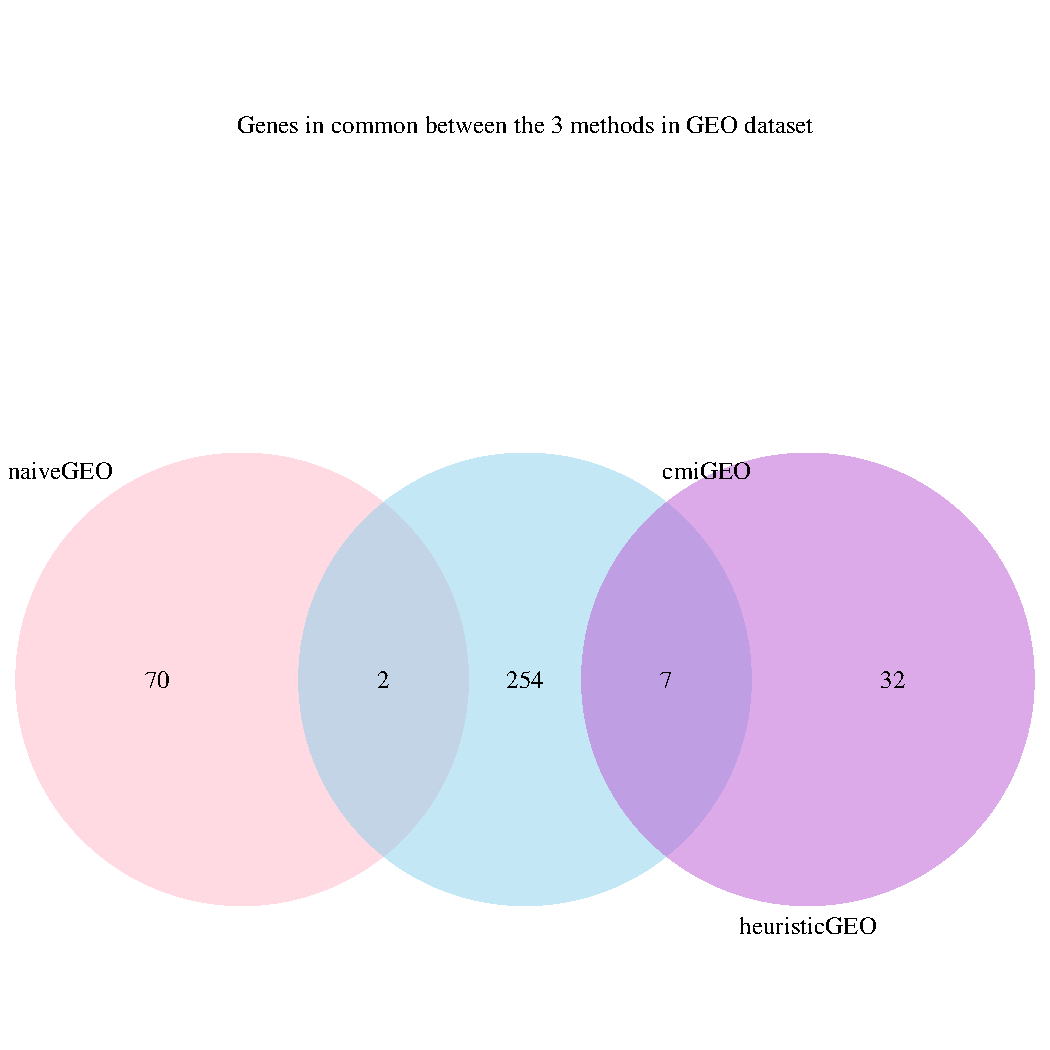
\includegraphics[width=\maxwidth]{figure/compare3GEO-1} 

\end{knitrout}

\begin{knitrout}
\definecolor{shadecolor}{rgb}{0.969, 0.969, 0.969}\color{fgcolor}\begin{kframe}
\begin{alltt}
\hlstd{myVenn3TCGA} \hlkwb{<-} \hlkwd{venn.diagram}\hlstd{(}\hlkwc{x}\hlstd{=}\hlkwd{list}\hlstd{(}\hlkwc{naiveTCGA}\hlstd{=}\hlkwd{rownames}\hlstd{(selectedNaiveTCGA),}
                                \hlkwc{cmiTCGA}\hlstd{=}\hlkwd{rownames}\hlstd{(selectedCmiTCGA),}
                                \hlkwc{heuristicTCGA} \hlstd{=} \hlkwd{rownames}\hlstd{(selectedHeuristicTCGA)),}
                                \hlkwc{filename}\hlstd{=}\hlkwa{NULL}\hlstd{,} \hlkwc{lty} \hlstd{=} \hlstr{"blank"}\hlstd{,}
                                \hlkwc{fill}\hlstd{=}\hlkwd{c}\hlstd{(}\hlstr{"pink1"}\hlstd{,} \hlstr{"skyblue"}\hlstd{,} \hlstr{"mediumorchid"}\hlstd{),}
                       \hlkwc{main}\hlstd{=}\hlstr{"Genes in common between the 3 methods in TCGA dataset"}\hlstd{)}
\hlkwd{grid.newpage}\hlstd{()}
\hlkwd{grid.draw}\hlstd{(myVenn3TCGA)}
\end{alltt}
\end{kframe}
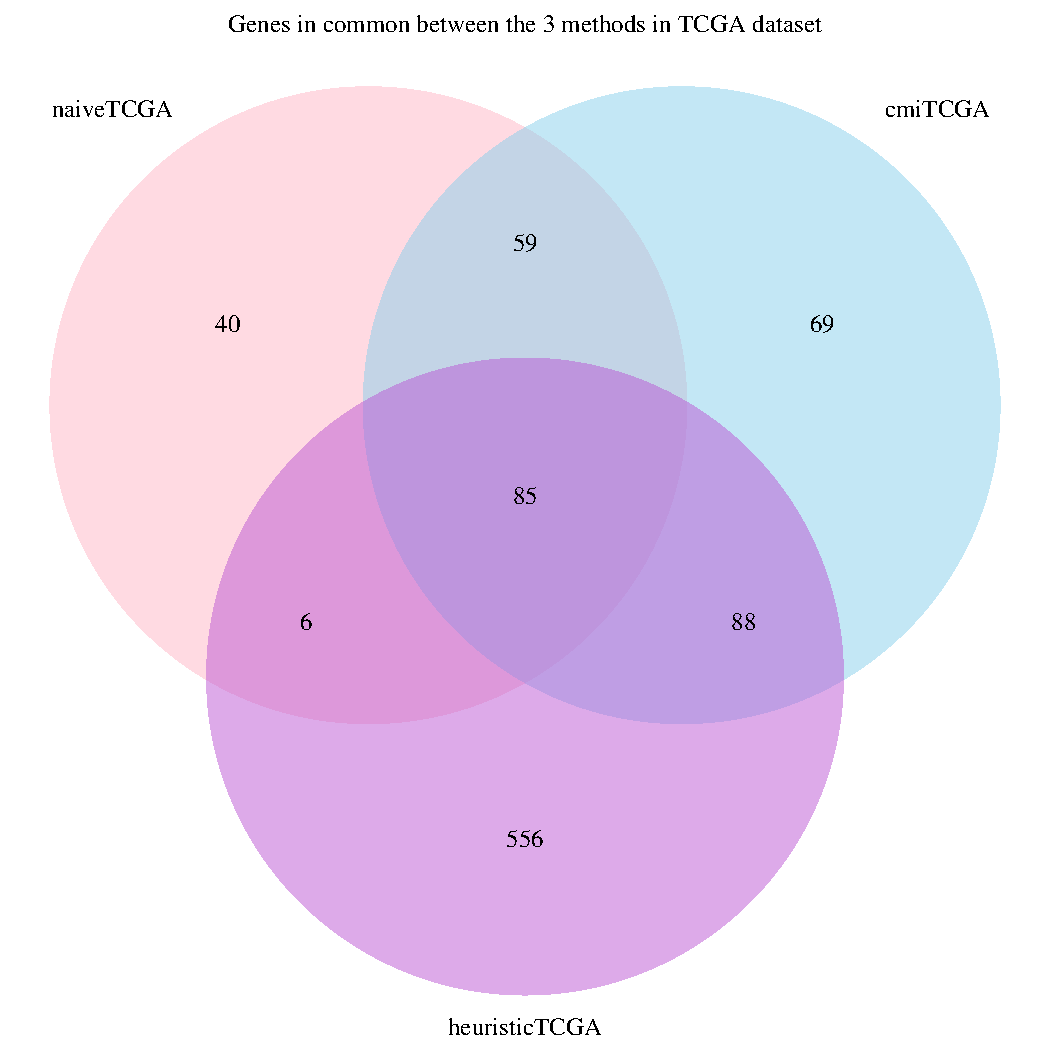
\includegraphics[width=\maxwidth]{figure/compare3TCGA-1} 

\end{knitrout}

\subsection{Common results}

A simple way to facilitat the comparison between the different scores and classifications provided by the distinct methods is simply to align these scores in a tabular format.

\begin{knitrout}
\definecolor{shadecolor}{rgb}{0.969, 0.969, 0.969}\color{fgcolor}\begin{kframe}
\begin{alltt}
\hlkwa{if} \hlstd{(}\hlopt{!}\hlkwd{exists} \hlstd{(}\hlstr{"naiveDA"}\hlstd{))}
  \hlkwd{load}\hlstd{(}\hlstr{"results/naiveSelections.Rda"}\hlstd{)}
\hlkwa{if} \hlstd{(}\hlopt{!}\hlkwd{exists} \hlstd{(}\hlstr{"cmiDA"}\hlstd{))}
  \hlkwd{load}\hlstd{(}\hlstr{"results/cmiSelections.Rda"}\hlstd{)}
\hlkwa{if} \hlstd{(}\hlopt{!}\hlkwd{exists} \hlstd{(}\hlstr{"scoresDA1"}\hlstd{))}
  \hlkwd{load}\hlstd{(}\hlstr{"results/heuristicSelections.Rda"}\hlstd{)}
\hlkwd{dim}\hlstd{(naiveDA);} \hlkwd{head}\hlstd{(naiveDA)}
\end{alltt}
\begin{verbatim}
## [1] 11359     5
\end{verbatim}
\end{kframe}


\begin{tabular}{l|r|r|r|r|l}
\hline
  & r (Sp) & p (Sp) & adj.Spear.Pval & distCor & SigNegCorr\\
\hline
A1BG & 0.1092 & 0.5656 & 0.8820 & 0.3175 & FALSE\\
\hline
A2M & -0.3700 & 0.0442 & 0.3391 & 0.4542 & FALSE\\
\hline
A2ML1 & -0.1355 & 0.4753 & 0.8455 & 0.2765 & FALSE\\
\hline
A4GALT & -0.3606 & 0.0503 & 0.3571 & 0.4278 & FALSE\\
\hline
A4GNT & -0.1657 & 0.3814 & 0.8017 & 0.2531 & FALSE\\
\hline
AAAS & -0.1293 & 0.4960 & 0.8541 & 0.2544 & FALSE\\
\hline
\end{tabular}\begin{kframe}\begin{alltt}
\hlkwd{dim}\hlstd{(cmiDA);} \hlkwd{head}\hlstd{(cmiDA)}
\end{alltt}
\begin{verbatim}
## [1] 11359     4
\end{verbatim}
\end{kframe}


\begin{tabular}{l|r|l|r|l}
\hline
  & cMI\_min & t\_opt & ratio & meth\_regulated\\
\hline
A1BG & 0.0003 & 0.69 & 0.0903 & FALSE\\
\hline
A2M & 0.0060 & 0.49 & 0.0726 & FALSE\\
\hline
A2ML1 & 0.0233 & 0.34 & 0.3245 & FALSE\\
\hline
A4GALT & 0.0338 & 0.34 & 0.3833 & FALSE\\
\hline
A4GNT & 0.0063 & 0.55 & 0.4343 & FALSE\\
\hline
AAAS & 0.0000 & 0 & 1.0000 & FALSE\\
\hline
\end{tabular}\begin{kframe}\begin{alltt}
\hlkwd{dim}\hlstd{(scoresDA1);} \hlkwd{head}\hlstd{(scoresDA1)}
\end{alltt}
\begin{verbatim}
## [1] 11359     2
\end{verbatim}
\end{kframe}


\begin{tabular}{l|l|r}
\hline
  & logicSc & numericSc\\
\hline
A1BG & FALSE & -78\\
\hline
A2M & FALSE & -20\\
\hline
A2ML1 & FALSE & 0\\
\hline
A4GALT & TRUE & 21\\
\hline
A4GNT & FALSE & -91\\
\hline
AAAS & FALSE & 0\\
\hline
\end{tabular}\begin{kframe}\begin{alltt}
\hlstd{DAvalues} \hlkwb{<-} \hlkwd{cbind}\hlstd{(naiveDA, cmiDA, scoresDA1);}
\hlkwd{head}\hlstd{(DAvalues)}
\end{alltt}
\end{kframe}


\begin{tabular}{l|r|r|r|r|l|r|l|r|l|l|r}
\hline
  & r (Sp) & p (Sp) & adj.Spear.Pval & distCor & SigNegCorr & cMI\_min & t\_opt & ratio & meth\_regulated & logicSc & numericSc\\
\hline
A1BG & 0.1092 & 0.5656 & 0.8820 & 0.3175 & FALSE & 0.0003 & 0.69 & 0.0903 & FALSE & FALSE & -78\\
\hline
A2M & -0.3700 & 0.0442 & 0.3391 & 0.4542 & FALSE & 0.0060 & 0.49 & 0.0726 & FALSE & FALSE & -20\\
\hline
A2ML1 & -0.1355 & 0.4753 & 0.8455 & 0.2765 & FALSE & 0.0233 & 0.34 & 0.3245 & FALSE & FALSE & 0\\
\hline
A4GALT & -0.3606 & 0.0503 & 0.3571 & 0.4278 & FALSE & 0.0338 & 0.34 & 0.3833 & FALSE & TRUE & 21\\
\hline
A4GNT & -0.1657 & 0.3814 & 0.8017 & 0.2531 & FALSE & 0.0063 & 0.55 & 0.4343 & FALSE & FALSE & -91\\
\hline
AAAS & -0.1293 & 0.4960 & 0.8541 & 0.2544 & FALSE & 0.0000 & 0 & 1.0000 & FALSE & FALSE & 0\\
\hline
\end{tabular}\begin{kframe}\begin{alltt}
\hlstd{GEOvalues} \hlkwb{<-} \hlkwd{cbind}\hlstd{(naiveGEO, cmiGEO, scoresGEO)}
\hlkwd{head}\hlstd{(GEOvalues)}
\end{alltt}
\end{kframe}


\begin{tabular}{l|r|r|r|r|l|r|l|r|l|l|r}
\hline
  & r (Sp) & p (Sp) & adj.Spear.Pval & distCor & SigNegCorr & cMI\_min & t\_opt & ratio & meth\_regulated & logicSc & numericSc\\
\hline
7A5 & 0.4346 & 0.0299 & 0.5629 & 0.4752 & FALSE & 0.0107 & 0.15 & 0.7215 & FALSE & FALSE & 0\\
\hline
A1BG & -0.0415 & 0.8437 & 0.9815 & 0.4135 & FALSE & 0.0202 & 0.91 & 0.4165 & FALSE & FALSE & -25\\
\hline
A2BP1 & 0.0762 & 0.7175 & 0.9675 & 0.1491 & FALSE & 0.0498 & 0.18 & 0.2377 & FALSE & FALSE & -31\\
\hline
A2ML1 & -0.1392 & 0.5068 & 0.9291 & 0.1918 & FALSE & 0.0567 & 0.3 & 0.4678 & FALSE & FALSE & -39\\
\hline
A4GALT & -0.1023 & 0.6265 & 0.9526 & 0.3119 & FALSE & 0.0104 & 0.22 & 0.5322 & FALSE & FALSE & 0\\
\hline
A4GNT & -0.4654 & 0.0191 & 0.4740 & 0.2552 & FALSE & 0.0319 & 0.44 & 0.1731 & TRUE & FALSE & -4\\
\hline
\end{tabular}\begin{kframe}\begin{alltt}
\hlstd{TCGAvalues} \hlkwb{<-} \hlkwd{cbind}\hlstd{(naiveTCGA, cmiTCGA, scoresTCGA)}
\hlkwd{head}\hlstd{(TCGAvalues)}
\end{alltt}
\end{kframe}


\begin{tabular}{l|r|r|r|r|l|r|l|r|l|l|r}
\hline
  & r (Sp) & p (Sp) & adj.Spear.Pval & distCor & SigNegCorr & cMI\_min & t\_opt & ratio & meth\_regulated & logicSc & numericSc\\
\hline
A1BG & -0.0784 & 0.2437 & 0.4304 & 0.1104 & FALSE & 0.0103 & 0.62 & 0.7452 & FALSE & FALSE & -1224.6\\
\hline
A2M & -0.1889 & 0.0046 & 0.0229 & 0.2023 & FALSE & 0.0121 & 0.69 & 0.4491 & FALSE & FALSE & -182.6\\
\hline
A2ML1 & -0.0203 & 0.7627 & 0.8700 & 0.1178 & FALSE & 0.0100 & 0.37 & 0.2897 & FALSE & TRUE & 113.0\\
\hline
A4GALT & -0.0866 & 0.1977 & 0.3758 & 0.1560 & FALSE & 0.0145 & 0.43 & 0.5731 & FALSE & FALSE & -102.6\\
\hline
A4GNT & 0.0893 & 0.1841 & 0.3586 & 0.1167 & FALSE & 0.0167 & 0.53 & 0.6076 & FALSE & FALSE & -274.4\\
\hline
AAAS & -0.1915 & 0.0041 & 0.0208 & 0.1989 & FALSE & 0.0021 & 0.21 & 0.5165 & FALSE & FALSE & 0.0\\
\hline
\end{tabular}\begin{kframe}\begin{alltt}
\hlkwd{write.csv}\hlstd{(DAvalues,} \hlkwc{file}\hlstd{=}\hlstr{"results/LshapeScoresDA.csv"}\hlstd{)}
\hlkwd{write.csv}\hlstd{(GEOvalues,} \hlkwc{file}\hlstd{=}\hlstr{"results/LshapeScoresGEO.csv"}\hlstd{)}
\hlkwd{write.csv}\hlstd{(TCGAvalues,} \hlkwc{file}\hlstd{=}\hlstr{"results/LshapeScoresTCGA.csv"}\hlstd{)}
\hlcom{# require(WriteXLS)}
\hlcom{# WriteXLS(x=c("DAvalues", "GEOvalues", "TCGAvalues"), ExcelFileName = "results/LshapeScores.xls")}
\end{alltt}
\end{kframe}
\end{knitrout}

\subsection{Plotting expression-methylation scaterplots}

The best way to decide if a gene can be called L--shaped is to look at the methylation--expression scatterplot.
Once we have computed the distinct scores we can combine these with the plots as shown below.

\begin{itemize}
  \item \texttt{DAExprAllScores.pdf}
  \item \texttt{DARNAseqLGenesScores.pdf}
  \item \texttt{GEOLGenesScores.pdf}
\end{itemize}

\begin{knitrout}
\definecolor{shadecolor}{rgb}{0.969, 0.969, 0.969}\color{fgcolor}\begin{kframe}
\begin{alltt}
\hlkwa{if} \hlstd{(}\hlopt{!}\hlstd{(}\hlkwd{exists}\hlstd{(}\hlstr{"DAMetilData"}\hlstd{)))}
  \hlkwd{load}\hlstd{(}\hlkwc{file}\hlstd{=}\hlstr{"dades/DataMatrices-DA.Rda"}\hlstd{)}
\hlkwa{if} \hlstd{(}\hlopt{!}\hlstd{(}\hlkwd{exists}\hlstd{(}\hlstr{"geoMetilData"}\hlstd{)))}
  \hlkwd{load}\hlstd{(}\hlkwc{file}\hlstd{=}\hlstr{"dades/DataMatrices-GEO.Rda"}\hlstd{)}
\hlkwa{if} \hlstd{(}\hlopt{!}\hlstd{(}\hlkwd{exists}\hlstd{(}\hlstr{"TCGAMetilData"}\hlstd{)))}
  \hlkwd{load}\hlstd{(}\hlkwc{file}\hlstd{=}\hlstr{"dades/DataMatrices-TCGA.Rda"}\hlstd{)}
\end{alltt}
\end{kframe}
\end{knitrout}

\begin{knitrout}
\definecolor{shadecolor}{rgb}{0.969, 0.969, 0.969}\color{fgcolor}\begin{kframe}
\begin{alltt}
\hlkwa{if} \hlstd{(}\hlopt{!}\hlkwd{exists}\hlstd{(}\hlstr{"DAvalues"}\hlstd{))}
  \hlstd{DAvalues}\hlkwb{<-} \hlkwd{read.csv}\hlstd{(}\hlkwc{file}\hlstd{=}\hlstr{"results/LshapeScoresDA.csv"}\hlstd{,} \hlkwc{row.names} \hlstd{=} \hlnum{1}\hlstd{)}
\hlstd{DAscores4plots} \hlkwb{<-} \hlstd{DAvalues[,}\hlkwd{c}\hlstd{(}\hlnum{1}\hlstd{,}\hlnum{3}\hlstd{,}\hlnum{10}\hlstd{,}\hlnum{11}\hlstd{)]}
\hlkwa{if} \hlstd{(}\hlopt{!}\hlkwd{exists}\hlstd{(}\hlstr{"GEOvalues"}\hlstd{))}
  \hlstd{GEOvalues}\hlkwb{<-} \hlkwd{read.csv}\hlstd{(}\hlkwc{file}\hlstd{=}\hlstr{"results/LshapeScoresGEO.csv"}\hlstd{,} \hlkwc{row.names} \hlstd{=} \hlnum{1}\hlstd{)}
\hlstd{GEOscores4plots} \hlkwb{<-} \hlstd{GEOvalues[,}\hlkwd{c}\hlstd{(}\hlnum{1}\hlstd{,}\hlnum{3}\hlstd{,}\hlnum{10}\hlstd{,}\hlnum{11}\hlstd{)]}
\hlkwa{if} \hlstd{(}\hlopt{!}\hlkwd{exists}\hlstd{(}\hlstr{"TCGAvalues"}\hlstd{))}
  \hlstd{TCGAvalues}\hlkwb{<-} \hlkwd{read.csv}\hlstd{(}\hlkwc{file}\hlstd{=}\hlstr{"results/LshapeScoresTCGA.csv"}\hlstd{,} \hlkwc{row.names} \hlstd{=} \hlnum{1}\hlstd{)}
\hlstd{TCGAscores4plots} \hlkwb{<-} \hlstd{TCGAvalues[,}\hlkwd{c}\hlstd{(}\hlnum{1}\hlstd{,}\hlnum{3}\hlstd{,}\hlnum{10}\hlstd{,}\hlnum{11}\hlstd{)]}
\hlstd{formatScores} \hlkwb{<-} \hlkwa{function}\hlstd{(}\hlkwc{x}\hlstd{)\{}
  \hlkwd{paste}\hlstd{(} \hlstr{"\textbackslash{}n"}\hlstd{,} \hlstr{"r(Sp)="}\hlstd{,} \hlkwd{round}\hlstd{(x[}\hlnum{1}\hlstd{],} \hlnum{4}\hlstd{) ,} \hlstr{"; adj-p="}\hlstd{,} \hlkwd{round}\hlstd{(x[}\hlnum{2}\hlstd{],}\hlnum{5}\hlstd{),}\hlstr{"\textbackslash{}n"}\hlstd{,} \hlstr{"Heur-L="}\hlstd{,} \hlkwd{as.logical}\hlstd{(x[}\hlnum{3}\hlstd{]),} \hlstr{"; Heur-score="}\hlstd{, x[}\hlnum{4}\hlstd{])}
  \hlstd{\}}

\hlstd{DAscores}\hlkwb{<-} \hlkwd{apply}\hlstd{(DAscores4plots,}\hlnum{1}\hlstd{, formatScores)} \hlcom{# head(DAscores)}
\hlstd{GEOscores}\hlkwb{<-} \hlkwd{apply}\hlstd{(GEOscores4plots,}\hlnum{1}\hlstd{, formatScores)} \hlcom{# head(GEOscores)}
\hlstd{TCGAscores}\hlkwb{<-} \hlkwd{apply}\hlstd{(TCGAscores4plots,}\hlnum{1}\hlstd{, formatScores)} \hlcom{# head(TCGAscores)}
\end{alltt}
\end{kframe}
\end{knitrout}

\begin{knitrout}
\definecolor{shadecolor}{rgb}{0.969, 0.969, 0.969}\color{fgcolor}\begin{kframe}
\begin{alltt}
\hlstd{replot} \hlkwb{<-} \hlnum{TRUE}
\hlkwa{if}\hlstd{(replot)\{}
      \hlkwd{plotGenesMat} \hlstd{(}\hlkwc{mets}\hlstd{=DAMetilData,}
              \hlkwc{expres}\hlstd{=DAExprData,}
              \hlkwc{fileName} \hlstd{=} \hlstr{"results/DAExprAllScores.pdf"}\hlstd{,}
              \hlkwc{text4Title} \hlstd{= DAscores)}
      \hlkwd{plotGenesMat} \hlstd{(}\hlkwc{mets}\hlstd{=geoMetilData,}
              \hlkwc{expres}\hlstd{=geoExprData,}
              \hlkwc{fileName} \hlstd{=}\hlstr{"results/GEOLGenesScores.pdf"}\hlstd{,}
              \hlkwc{text4Title} \hlstd{= GEOscores)}
      \hlkwd{plotGenesMat} \hlstd{(}\hlkwc{mets}\hlstd{=TCGAMetilData,}
              \hlkwc{expres}\hlstd{=TCGAExprData,}
              \hlkwc{fileName} \hlstd{=} \hlstr{"results/TCGALGenesScores.pdf"}\hlstd{,}
              \hlkwc{text4Title} \hlstd{= TCGAscores)}
  \hlstd{\}}
\end{alltt}
\begin{verbatim}
## pdf 
##   2
\end{verbatim}
\end{kframe}
\end{knitrout}


\section{Locating genes along the genome}

It is known that methylation happens at some specific regions in the genome (``cpG islands'') more often than in other places (sometimes called ``oceans'').
We would like to know if genes that have been found to be regulated by methylation \emph{in this study} are located at random in the genome or, alternatively, they concentrate in specific regions.

Altogether after applying the three methods --naive, cmi, heuristic-- to the three datasets --DA, GEO, TCGA-- we have selected 9 gene lists. 

\subsection{Annotating the genes in the chromosomes}

Each gene list can be annotated with the positions of the genes in the chromosomes using the human reference genome assembly \texttt{hg19}, of UCSC (University of California, Santa Cruz) through the bioconductor packages, \texttt{Homo.sapiens} and \texttt{TxDb.Hsapiens.UCSC.hg19.knownGene}.


For each method and dataset the transcript coordinates have been obtained, saved to binary files \texttt{transcriptCoords-\emph{Method-Dataset}.Rda} and written to .csv files \texttt{transcriptCoords-\emph{Method-Dataset}.csv} in the folder \texttt{results}, where \emph{Method} may be \texttt{Naive, CMI, Heuristic} and \texttt{Dataset} may be {DA, GEO, TCGA}.



For example the table of annotations corresponding to the \texttt{selectedNaiveDA} gene list has the following aspect:

\begin{knitrout}
\definecolor{shadecolor}{rgb}{0.969, 0.969, 0.969}\color{fgcolor}


\begin{tabular}{l|l|l|r|l|l|r|r}
\hline
  & ENTREZID & SYMBOL & TXNAME & TXID & TXCHROM & TXSTART & TXEND\\
\hline
31 & 10103 & TSPAN1 & 1244 & uc001cpd.3 & chr1 & 46640749 & 46651634\\
\hline
41 & 10158 & PDZK1IP1 & 5278 & uc001cqw.3 & chr1 & 47649261 & 47655771\\
\hline
57 & 10472 & ZBTB18 & 3989 & uc031psv.1 & chr1 & 244212241 & 244220780\\
\hline
61 & 10763 & NES & 6755 & uc001fpq.3 & chr1 & 156638556 & 156647189\\
\hline
81 & 11000 & SLC27A3 & 2533 & uc001fcz.3 & chr1 & 153747768 & 153752633\\
\hline
171 & 1382 & CRABP2 & 6756 & uc001fpr.3 & chr1 & 156669400 & 156675459\\
\hline
\end{tabular}
\end{knitrout}


\subsection{Visualization of selected genes in the chromosomes}

%%%%%%%%%%%%%%%%%%%%%%%%%%%%%%%%%%%%%%%%%%%%%%%%%%%%%%%%%%%%%%%%%%%%%%%%%%%%%
% HO HE DEIXAT A FALSE PQ HI INTERVENEN ARXIUS GRANS QUE NO TINC A GITHUB
%%%%%%%%%%%%%%%%%%%%%%%%%%%%%%%%%%%%%%%%%%%%%%%%%%%%%%%%%%%%%%%%%%%%%%%%%%%%%%

An interesting question when selecting genes putatively regulated by Methylation is if the genes are located at random or if they are clustered or grouped according to some criterion.

Two distinct classes of objects can be reasonably related with methylated genes: \texttt{CpG Islands} and \emph{DNAse I Hypersensitive Sites (DHS)}. 
\begin{enumerate}
\item CpG islands are said to mark important regions in the genome because over 65\% of gene promoter regions can be found within CpG islands. A dataset with the model CpG island mapped onto the hg19 genome can be obtained from the USCS (\url{http://hgdownload.cse.ucsc.edu/goldenpath/hg19/database/cpgIslandExt.txt.gz})
\item DNAse I hypersensitive sites are regions of chromatin that are sensitive to cleavage by the DNase I enzyme. Since the discovery of DHSs 30 years ago, they have been used as markers of regulatory DNA regions. In these specific regions of the genome, chromatin has lost its condensed structure, exposing the DNA and making it accessible. This raises the availability of DNA to degradation by enzymes, such as DNase I. These accessible chromatin zones are functionally related to transcriptional activity, since this remodeled state is necessary for the binding of proteins such as transcription factors. See \url{https://en.wikipedia.org/wiki/DNase_I_hypersensitive_site}. DHs can be downloaded from: \url{http://hgdownload.cse.ucsc.edu/goldenpath/hg19/encodeDCC/wgEncodeRegDnaseClustered/}.
\end{enumerate}

In order to facilitate the study of the relation between these objects and the genes regulated by methylation CpG islands and DH sites  will be plotted along the genome jointly with the selected genes.

The resulting plots will be printed to pdf files  \texttt{Genes2Chromosomes-\emph{Method-Dataset}.pdf} in the folder \texttt{results}, where \emph{Method} may be \texttt{Naive, CMI, Heuristic} and \texttt{Dataset} may be {DA, GEO, TCGA}

\subsubsection{Preparing data sources information}

As a first step to plotting the coordinates of the \emph{necessary} CpG islands and DH sites are obtained. By ``necessary'' we mean only those that correspond to positions located between the first transcript and the last transcripts associated with selected genes. Information is read from public files and stored in objects of type \texttt{GRanges}, a Bioconductor class to efficiently store information about sequences.



Next for each set of transcripts coordinates 

\begin{knitrout}
\definecolor{shadecolor}{rgb}{0.969, 0.969, 0.969}\color{fgcolor}\begin{kframe}
\begin{alltt}
\hlstd{redraw} \hlkwb{<-} \hlnum{TRUE}
\hlkwa{if} \hlstd{(redraw)\{}
  \hlkwa{for} \hlstd{(i} \hlkwa{in} \hlnum{1}\hlopt{:}\hlkwd{length}\hlstd{(transcriptCoordsList))\{}
    \hlkwd{plotGenesInChroms} \hlstd{(transcriptCoordsList[[i]],}
                       \hlkwd{paste}\hlstd{(}\hlstr{"results/genePositions"}\hlstd{,} \hlkwd{names}\hlstd{(transcriptCoordsList)[i],}\hlstr{".pdf"}\hlstd{,} \hlkwc{sep}\hlstd{=}\hlstr{""}\hlstd{),}
                       \hlkwc{minbase}\hlstd{=minbase,} \hlkwc{maxbase}\hlstd{=maxbase,} \hlkwc{islandData}\hlstd{=islandData,} \hlkwc{dnaseData}\hlstd{=dnaseData)}
  \hlstd{\}}
\hlstd{\}}
\end{alltt}
\end{kframe}
\end{knitrout}

Figure \ref{chromosome1} shows the genes selected using the Naive method on the DA dataset in the first chromosome only.

\begin{knitrout}
\definecolor{shadecolor}{rgb}{0.969, 0.969, 0.969}\color{fgcolor}\begin{kframe}
\begin{alltt}
\hlcom{# Select columns needed for plotting  }
\hlstd{anotacs4}\hlkwb{<-}\hlstd{transcriptCoordsList[[}\hlnum{1}\hlstd{]][,}\hlkwd{c}\hlstd{(}\hlstr{'TXCHROM'}\hlstd{,} \hlstr{'TXSTART'}\hlstd{,} \hlstr{'TXEND'}\hlstd{)]}
\hlstd{anotacs4}\hlkwb{<-}\hlstd{anotacs4[}\hlkwd{complete.cases}\hlstd{(anotacs4),]}
\hlcom{#change column names to read it into GenomicRanges}
\hlkwd{colnames}\hlstd{(anotacs4)}\hlkwb{<-}\hlkwd{c}\hlstd{(}\hlstr{"chromosome"}\hlstd{,}\hlstr{"start"}\hlstd{,}\hlstr{"end"}\hlstd{)}
\hlstd{genRangList}\hlkwb{<-}\hlkwd{makeGRangesFromDataFrame}\hlstd{(anotacs4)} \hlcom{#if we keep geneid we add keep.extra.columns=TRUE inside function}
\hlcom{# load context information necessary for plotting}
\hlstd{data} \hlkwb{<-} \hlkwd{read.table}\hlstd{(}\hlkwd{paste}\hlstd{(}\hlstr{"dades"}\hlstd{,}\hlstr{"cytoBandIdeo.txt"}\hlstd{,} \hlkwc{sep}\hlstd{=}\hlstr{"/"}\hlstd{),} \hlkwc{header}\hlstd{=F,} \hlkwc{sep}\hlstd{=}\hlstr{"\textbackslash{}t"}\hlstd{)}
\hlkwd{colnames}\hlstd{(data)} \hlkwb{<-}\hlkwd{c}\hlstd{(}\hlstr{'chrom'}\hlstd{,} \hlstr{'chromStart'}\hlstd{,} \hlstr{'chromEnd'}\hlstd{,} \hlstr{'name'}\hlstd{,} \hlstr{'gieStain'}\hlstd{)}
\hlstd{ideoTrack} \hlkwb{<-} \hlkwd{IdeogramTrack}\hlstd{(}\hlkwc{genome}\hlstd{=}\hlstr{"mm10"}\hlstd{,}\hlkwc{chromosome} \hlstd{=} \hlstr{"chr2"}\hlstd{,} \hlkwc{bands}\hlstd{=data)}

\hlcom{# Go to plotting}
\hlstd{axisT}\hlkwb{<-}\hlkwd{GenomeAxisTrack}\hlstd{()}
\hlstd{genList1}\hlkwb{<-}\hlkwd{AnnotationTrack}\hlstd{(anotacs4,} \hlkwc{name} \hlstd{=} \hlstr{"Genes"}\hlstd{,} \hlkwc{genome} \hlstd{=}\hlstr{"hg19"}\hlstd{,} \hlkwc{chromosome} \hlstd{=}\hlstr{"chr1"}\hlstd{,}
                          \hlkwc{stacking} \hlstd{=}\hlstr{"dense"}\hlstd{,} \hlkwc{col}\hlstd{=} \hlstr{"#5E2366"}\hlstd{,} \hlkwc{fill}\hlstd{=} \hlstr{"#5E2366"} \hlstd{)}
\hlstd{ideoT1}\hlkwb{<-}\hlkwd{IdeogramTrack}\hlstd{(}\hlkwc{genome}\hlstd{=}\hlstr{"hg19"}\hlstd{,} \hlkwc{bands} \hlstd{= data,}\hlkwc{chromosome} \hlstd{=} \hlstr{"chr1"}\hlstd{,} \hlkwc{showId}\hlstd{=}\hlnum{FALSE}\hlstd{)}
\hlstd{islandData1} \hlkwb{<-} \hlstd{islandData[}\hlkwd{seqnames}\hlstd{(islandData)} \hlopt{==} \hlstr{"chr1"} \hlopt{&}  \hlstd{(}\hlkwd{start}\hlstd{(islandData)} \hlopt{>=} \hlstd{minbase} \hlopt{&} \hlkwd{end}\hlstd{(islandData)} \hlopt{<=} \hlstd{maxbase)]}
\hlstd{islandTrack1} \hlkwb{<-} \hlkwd{AnnotationTrack}\hlstd{(}\hlkwc{range}\hlstd{=islandData1,} \hlkwc{genome}\hlstd{=}\hlstr{"hg19"}\hlstd{,} \hlkwc{name}\hlstd{=}\hlstr{"CpG Islands"}\hlstd{,}
                               \hlkwc{chromosome}\hlstd{=}\hlstr{"chr1"}\hlstd{)}
\hlcom{# DNaseI hypersensitive site data track}
\hlstd{dnaseTrack1} \hlkwb{<-} \hlkwd{DataTrack}\hlstd{(}\hlkwc{range}\hlstd{=dnaseData,} \hlkwc{genome}\hlstd{=}\hlstr{"hg19"}\hlstd{,} \hlkwc{name}\hlstd{=}\hlstr{"DNAseI"}\hlstd{,}
                        \hlkwc{type}\hlstd{=}\hlstr{"gradient"}\hlstd{,} \hlkwc{chromosome}\hlstd{=}\hlstr{"chr1"}\hlstd{)}
\hlkwd{pdf}\hlstd{(}\hlkwc{file}\hlstd{=}\hlstr{"results/chromosome1NaiveDA.pdf"}\hlstd{,} \hlkwc{width}\hlstd{=} \hlnum{8}\hlstd{,} \hlkwc{height} \hlstd{=} \hlnum{12}\hlstd{)}
  \hlkwd{plotTracks}\hlstd{(}\hlkwd{list}\hlstd{(ideoT1,axisT,genList1, dnaseTrack1, islandTrack1),}
             \hlkwc{sizes}\hlstd{=}\hlkwd{c}\hlstd{(}\hlnum{1}\hlstd{,}\hlnum{2}\hlstd{,}\hlnum{2}\hlstd{,}\hlnum{1}\hlstd{,}\hlnum{20}\hlstd{),} \hlkwc{main}\hlstd{=}\hlstr{"chr1"}\hlstd{,} \hlkwc{cex.main}\hlstd{=}\hlnum{1}\hlstd{,}  \hlkwc{littleTicks} \hlstd{=} \hlnum{TRUE}\hlstd{,} \hlkwc{showTitle}\hlstd{=}\hlnum{TRUE}\hlstd{)}
\hlkwd{dev.off}\hlstd{()}
\end{alltt}
\end{kframe}
\end{knitrout}

\begin{figure}
%\includegraphics{results/chromosome1NaiveDA.pdf}
\caption{\label{chromosome1} Distribution of genes on Chromosome 1. The genes are plotted as vertical purple lines, blue lines are the DNAse I hypersensitive sites and grey lines represent an accumulation of CpG islands.}
\end{figure}

\subsection{Overlap between CpG islands and selected genes}

Additionally to drawing genes and CpG regions together one can find out the overlap between gene regions and CpG islands.
This can be done by calling ``CpG islands'' genomic windows whose GC content>50\% and observed-to-expected CG ratio>0.6.

The overlap can be computed based on two methods: ``standadrd'' and ``within'' defined in the documentation of Bioconductor \texttt{GRanges} package.

For example, for the first chromosome and the gene list obtained by the Naive method on DA dataset we have:

\begin{knitrout}
\definecolor{shadecolor}{rgb}{0.969, 0.969, 0.969}\color{fgcolor}\begin{kframe}
\begin{alltt}
\hlcom{#Subset CpG islands and create a new GRanges object }
\hlstd{islandHMM2} \hlkwb{<-} \hlstd{islandHMM[islandHMM}\hlopt{$}\hlstd{GCcontent}\hlopt{>}\hlnum{50} \hlopt{&} \hlstd{islandHMM}\hlopt{$}\hlstd{obsExp}\hlopt{>}\hlnum{0.6}\hlstd{,]}

\hlstd{islandDataSel} \hlkwb{<-} \hlkwd{GRanges}\hlstd{(}\hlkwc{seqnames}\hlstd{=}\hlkwd{Rle}\hlstd{(islandHMM2}\hlopt{$}\hlstd{chr),}
                      \hlkwc{ranges}\hlstd{=}\hlkwd{IRanges}\hlstd{(}\hlkwc{start}\hlstd{=islandHMM2}\hlopt{$}\hlstd{start,} \hlkwc{end}\hlstd{=islandHMM2}\hlopt{$}\hlstd{end),}
                      \hlkwc{strand}\hlstd{=}\hlkwd{Rle}\hlstd{(}\hlkwd{strand}\hlstd{(}\hlkwd{rep}\hlstd{(}\hlstr{"*"}\hlstd{,}\hlkwd{nrow}\hlstd{(islandHMM2)))))}
\hlcom{## Overlapping two GRanges objects:}
\hlkwd{table}\hlstd{(}\hlopt{!}\hlkwd{is.na}\hlstd{(}\hlkwd{findOverlaps}\hlstd{(islandDataSel, genRangList,} \hlkwc{select}\hlstd{=}\hlstr{"arbitrary"}\hlstd{)))}
\hlstd{countFeatOverlaps} \hlkwb{<-} \hlkwd{countOverlaps}\hlstd{(islandDataSel, genRangList)}
\hlstd{findFeatOverlaps} \hlkwb{<-} \hlkwd{findOverlaps}\hlstd{(islandDataSel, genRangList)}
\hlstd{subsetFeatOverlaps} \hlkwb{<-} \hlkwd{subsetByOverlaps}\hlstd{(islandDataSel, genRangList)}
\hlstd{findFeatOverlapsWITHIN} \hlkwb{<-} \hlkwd{findOverlaps}\hlstd{(genRangList, islandDataSel,} \hlkwc{type}\hlstd{=}\hlstr{"within"}\hlstd{)}
\end{alltt}
\end{kframe}
\end{knitrout}

%The overlaps between the model CpG islands identified on the human genome and the genes identified from our query dataset (Naive-DA) were selected by 2 different methods with the following results:
%For a non-defined overlap, there were length(findFeatOverlaps) overlaps between the model CpG islands and the genes selected from the DA data; and for a within feature overlap, there were length(findFeatOverlapsWITHIN) overlaps.   

\clearpage
\begin{thebibliography}{9}

%\addcontentsline{toc}{chapter}{\numberline{}References}

\bibitem{bazzocco:2014} Sarah Bazzocco, Hafid Alazzouzi, M. Carme Ruiz de Villa, Alex Sanchez-Pla, John M. Mariadason, Diego Arango (2013) \emph{Genome-Wide Analysis of DNA Methylation in Colorectal Cancer}. Submitted.

\bibitem{Liu:2012} Yihua Liu and Peng Qiu. (2012) \emph{Integrative analysis of methylation and gene expression data in TCGA} IEEE International Workshop on Genomic Signal Processing and Statistics (GENSIPS)

\bibitem{r-project} R Development Core Team (2005). R: A language and environment for statistical computing,  reference index version 2.14.0. R Foundation for Statistical Computing, Vienna, Austria. ISBN 3-900051-07-0, \\
  \verb|http://www.R-project.org|

\bibitem{racine:2012} Jeffrey Racine. (2012) A primer on regression splines.\newline
\verb|http://cran.r-project.org/web/packages/crs/vignettes/spline_primer.pdf|

\end{thebibliography}

\end{document}
